\chapter{Effects of localised shearing on crystal growth and nucleation}
As outlined in Chapter 1, the original outline of the PhD was to investigate 
the possibility of using optical tweezing as a means of initiating and 
controlling nucleation by generating fluid flow within a small droplet of 
supersaturated solution. The goal of which would be to understand the 
influence of shearing on nucleation at a micro level as compared to larger 
scale results. It has been shown that for macro-scale systems, the likelihood 
of nucleation increases to a maximum value under increased shearing 
\cite{Debuysschere2023, Mura2016}. Theoretical research into the matter 
identified two competing effects that effect a crystal in moving fluid fields; 
firstly, nucleation is enhanced due to the increased mass transfer of solute 
material; and secondly, shear flow against the crystal surface leading to a 
decrease in growth \cite{Mura2016}. These two competing effects are validated 
by experimental work using glycine solutions, showing that beyond a certain 
shear rate the nucleation rate is reduced \cite{Debuysschere2023}. In this 
chapter I outline the optical tweezer equipment used during this PhD, the 
initial attempts made to induce nucleation via optical rotation, and the 
impact of a moving beam on the crystal growth of a newly formed nucleus.
%%%%%%%%%%%%%%%%%%%%%%%%%%%%%%%%%%%%%%%%%%%%%%%%%%%%%%%%%%%%%%%%%%%%%%%%%%%%%%%%
%%%%%%%%%%%%%%%%%%%%%%%%%%%%%%%%%%%%%%%%%%%%%%%%%%%%%%%%%%%%%%%%%%%%%%%%%%%%%%%% 
\section{Optical Tweezer Equipment}
In general, all optical tweezers require a laser driver, two
microscope objectives (one for trapping and one for imaging),
and a means of controlling the position of the loaded sample. 
While there are other pieces of equipment used in modern tweezer
experiments these are the bare minimum requirements for any 
optical tweezer. The laser used for this project was a 1064 
nm near infrared laser - provided by CNI Lasers – that has 
an adjustable power supply to vary the energy output of the 
laser - the remaining optics where supplied by Thor Labs.
Experimental work has shown that the trapping efficiency 
increases with beam diameter up until it exceeds $\frac{2}{3}D_{obj}$ 
\cite{kim2003dependence} where $D_{obj}$ is the diameter
of the objective aperture. To expand the beam front we 
utilise a Galilean beam expansion arrangement (indicated 
by $f_1$, and $f_2$) as recommended for high power laser 
applications. In our initial experiments the beam expansion 
provides a $4\times$ magnification; however, in later experiments 
where we utilise a galvano-mirror the beam expansion is $3\times$ 
and then the 4f correlator provides a further $1.25\times$ magnification 
(using $f_3$ and $f_4$) - where the magnification is given by.
\begin{align}
	\frac{D_2}{D_1} = \frac{f_2}{f_1}
\end{align}

It should be noted that the galvano-mirror requires the use 
of a Keplerian beam expansion arrangement which reduces
the transmitted laser power due to localised heating of the air.
Afterwards the laser is passed through a dichroic mirror that 
separates incoming infrared and visible light, this is to 
prevent the laser from damaging the CCD camera used for imaging
the trapping plane. The laser is then focused to a diffraction
limited spot by a 1.25 NA objective. By increasing the numerical
aperture of the objective, the gradient force at the focal point 
is increased; the trade-off being that the for higher NA values 
the trapping depth is reduced due to spherical aberrations.
While it is possible to increase the trapping depth \cite{Reihani2006} 
by adjusting the objective's tube length this approach is incompatible 
with our trapping arrangement. A 0.25 NA condenser objective refocuses
the scattered laser light and also provide an aperture for an 
imaging LED to illuminate the focal plane. Samples are loaded 
onto a piezo driven table to that is inserted between the trapping
and condensing objectives; the piezo drivers allow for sub-micron
control of the sample position to a degree as small as a 10 nm. 
To detect and monitor the position of a trapped particle a 
quadrant photo diode (QPD) was utilised. 
\begin{figure}[h!]
	\centering
	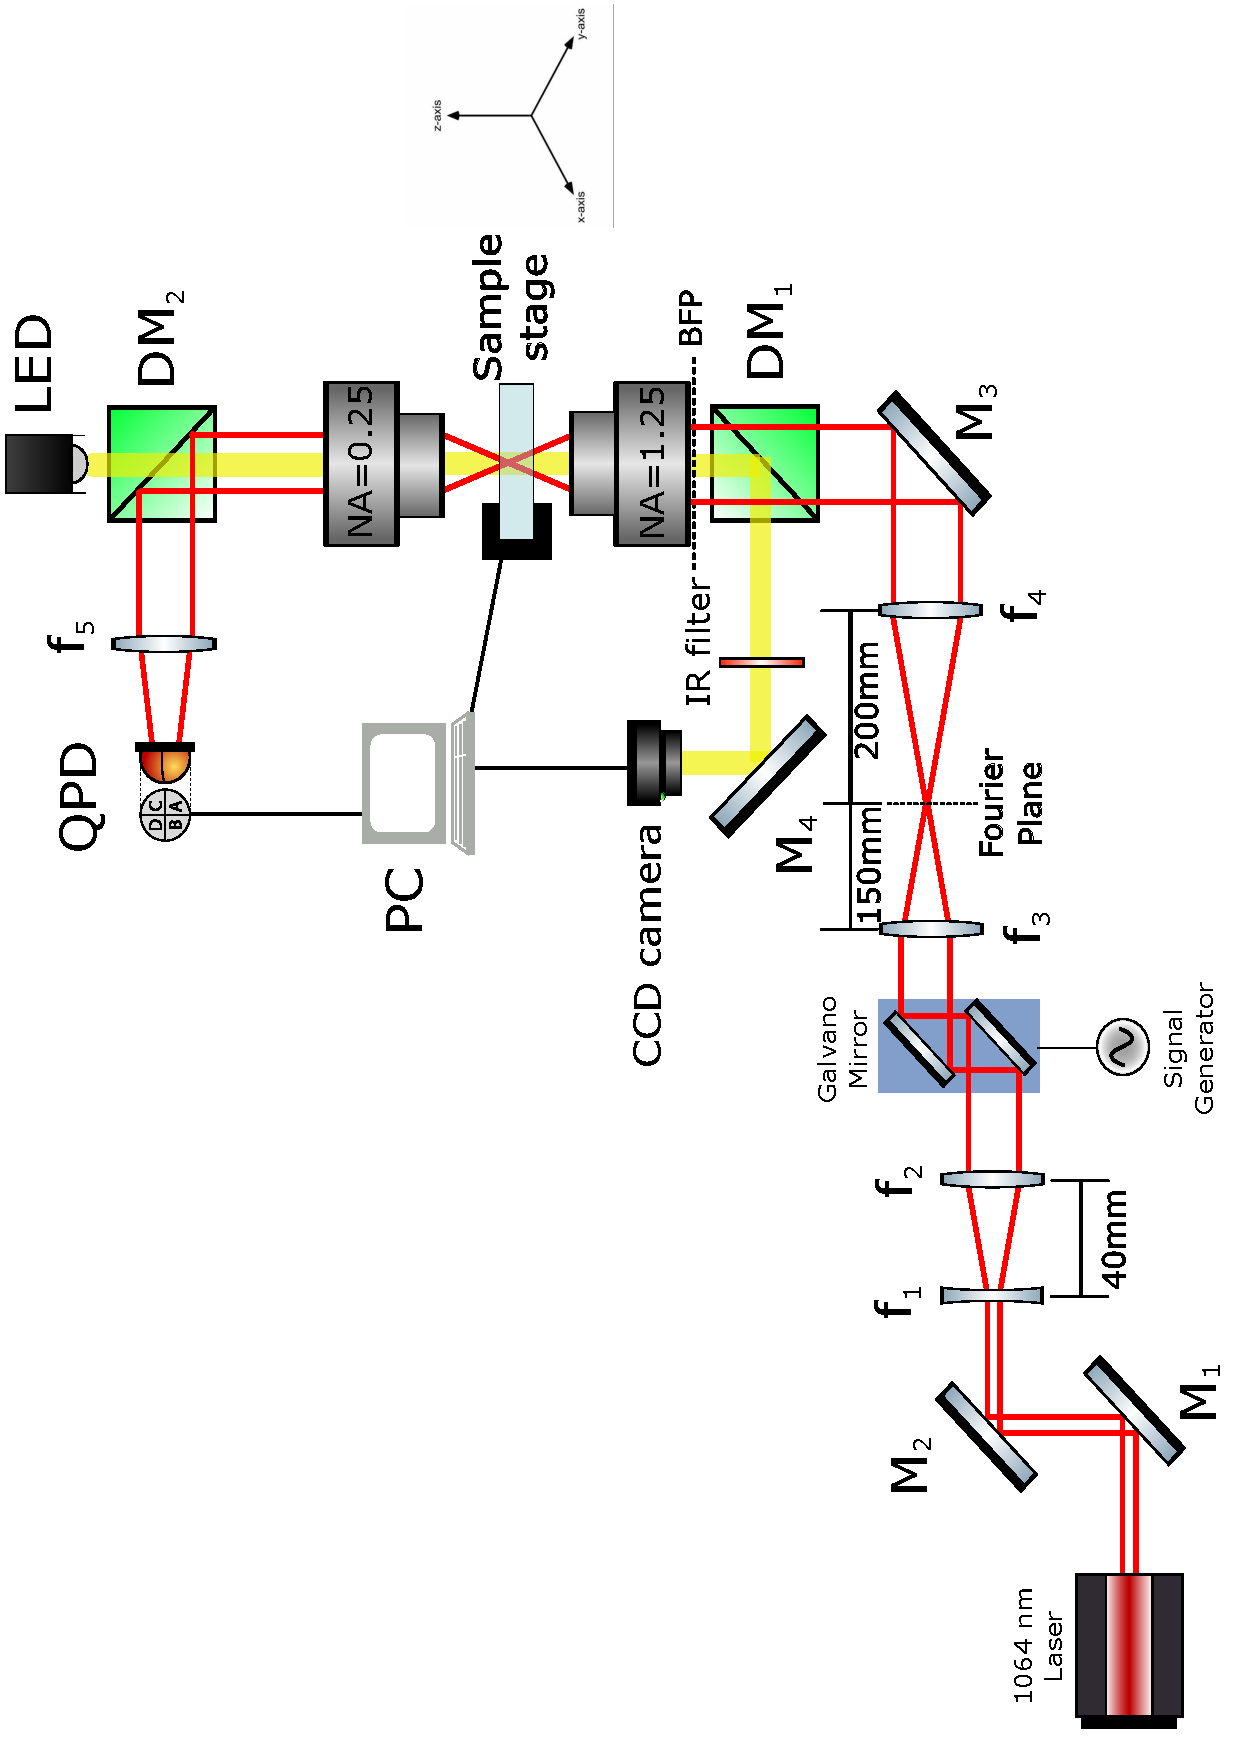
\includegraphics[height=\linewidth, angle=270]{tweezer_setup.pdf}
	\caption{Optical tweezer set up used for the majority of the PhD. The focal lengths of $f_1$, $f_2$, $f_3$, \& $f_4$ are $-20\ mm$, $60\ mm$, $150\ mm$, \& $200\ mm$ respectively. Diagram not drawn to scale.}
	\label{fig:setup}
\end{figure}

%%%%%%%%%%%%%%%%%%%%%%%%%%%%%%%%%%%%%%%%%%%%%%%%%%%%%%%%%%%%%%%%%%%%%%%%%%%%%%%%
\subsection{Position detection methods}
In order to accurately capture the dynamics of a trapped particle, 
a position detection system is utilised. There are 3 possible
methods of position detection: video-analysis, lateral-effect
position sensing, and photodiodes. The former being 
ideally suited for multiple traps or situations where precision
is not the top priority. In order to match the force measurements
of back-focal plane interferometry requires the camera's frame
rate to exceed $1\ kHz$ which can be difficult to achieve while 
maintaining a decent resolution \cite{Gibson2008}. In comparison
off the shelf back-focal plane detectors can achieve temporal
resolutions anywhere from $10-100\ kHz$ \cite{BergSoerensen2004}. 
 
A QPD is frequently used position detection system for optical 
tweezers due to their high sampling rate, high degree of 
precision, and ease of set up. The QPD is constructed of four photo 
diodes assembled in a quadrant formation, when a particle is trapped the 
interference pattern produced is focused onto the QPD, with 
the maximum intensity mapping to the particle's centre of mass. 
By summing the voltages of the horizontal and vertical quadrants 
together the particle's centre of mass is tracked in the x-y 
plane. Axial displacement can be estimated by observing the change
in the total voltage of the QPD. The outputted signal gives an
indication of the particle's relative displacement from the beam 
focus, but in order to convert the signal to distance units the
trap needs to be calibrated (assuming a linear response curve).
\begin{figure}[h!]
	\centering
	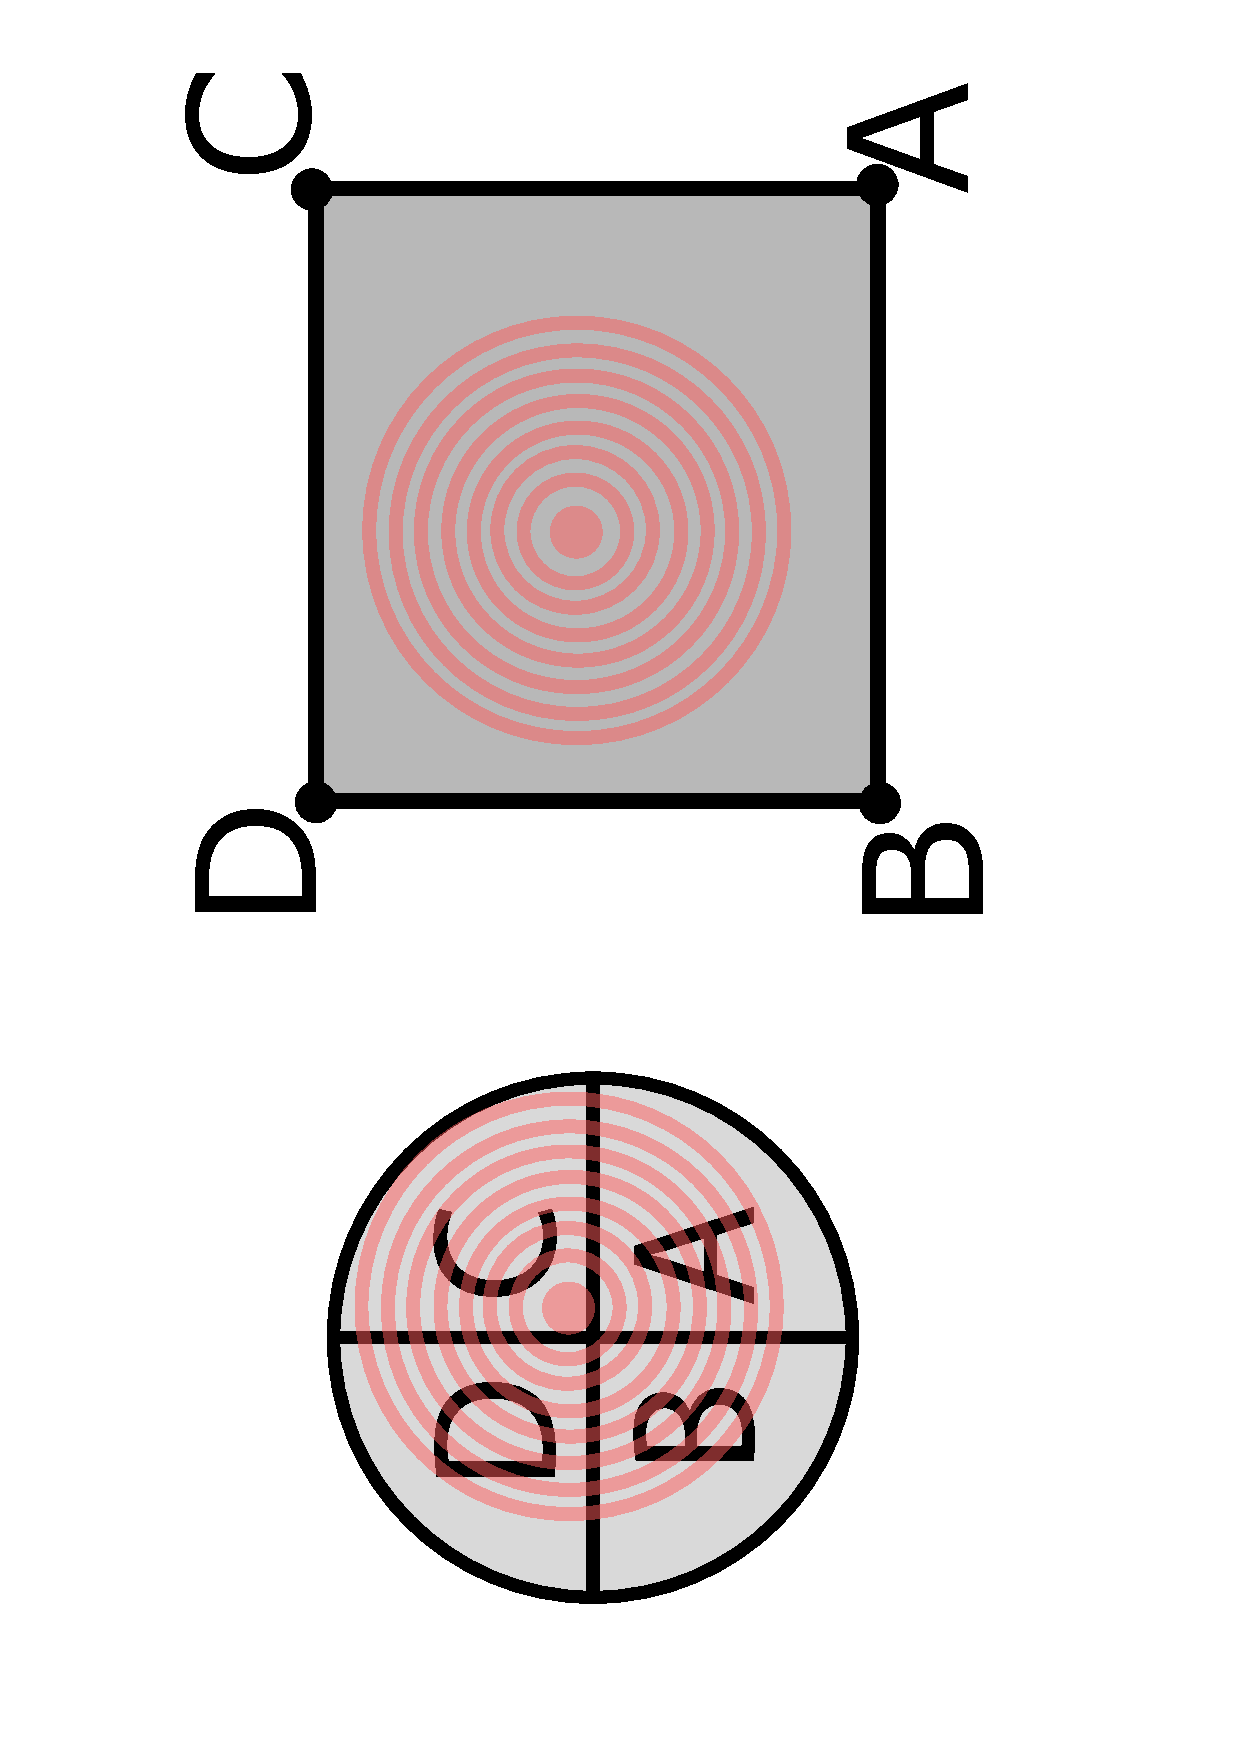
\includegraphics[height=\linewidth, angle=270]{QPD_Lateral_effect.pdf}
	\caption{Comparison between QPD and Lateral effect photodiodes.
	The four quadrants of a QPD (left) experience different photocurrents
	based on the total intensity of light incident on each section 
	(labelled A, B, C, D). 
	Whereas a Lateral effect sensor (right) uses the resistive properties
	of the photodiode surface to vary the create different photocurrents 
	passing through the anodes A, B, C, and D.}
\end{figure}

A lateral-effect sensor has a similar output but works using a 
the entire sensor as a single cell analogous to the focal plane of
the trapping beam. The four corners of the sensor act as anodes 
connected to a base plate cathode, as the beam moves across the
surface of the detector each anode will experience a different 
photocurrent depending on how close the centre of the 
interference pattern is to each anode. The advantage of a 
lateral effect detector is that the linear regime is much larger 
than a QPD making it much better for monitoring the position of a
trapped particle. However, Lateral-effect sensors are often limited
in their spacial resolution due to high signal-to-noise ratios, 
requiring a high intensity of light on the sensor in order to 
get a clean signal. As a result, most optical trapping experiments
are conducted using a QPD as opposed to a lateral-effect sensor, 
as often the displacement is small enough that the QPD response 
curve can be considered linear.

%%%%%%%%%%%%%%%%%%%%%%%%%%%%%%%%%%%%%%%%%%%%%%%%%%%%%%%%%%%%%%%%%%%%%%%%%%%%%%%%
\subsection{Fourier Optics and 4f correlators}
A 4f correlator is an example of Fourier optics in practice, understanding
that a focused lens takes a Fourier transform of the light profile. 
Consider a laser with a circular Gaussian profile, if you were to place 
a detector there you would pick up the intensity as a function of its 
position within the beam. If however you focused the light into a single 
point (using a +ve focal lens) you are actually seeing a measurement of 
the phase of your laser with position, in which you would see a diffraction
limited spot ($d = \lambda/2nsin(\theta)$), indicating that the laser is 
collimated. In imaging systems, a series of focal lenses can be used to 
filter out unwanted scattering from an image (or in an inverse case 
differentiate between different images), the placement of each lens is shown below.
\begin{figure}[h!]
	\centering
	\begin{subfigure}{0.475\linewidth}
		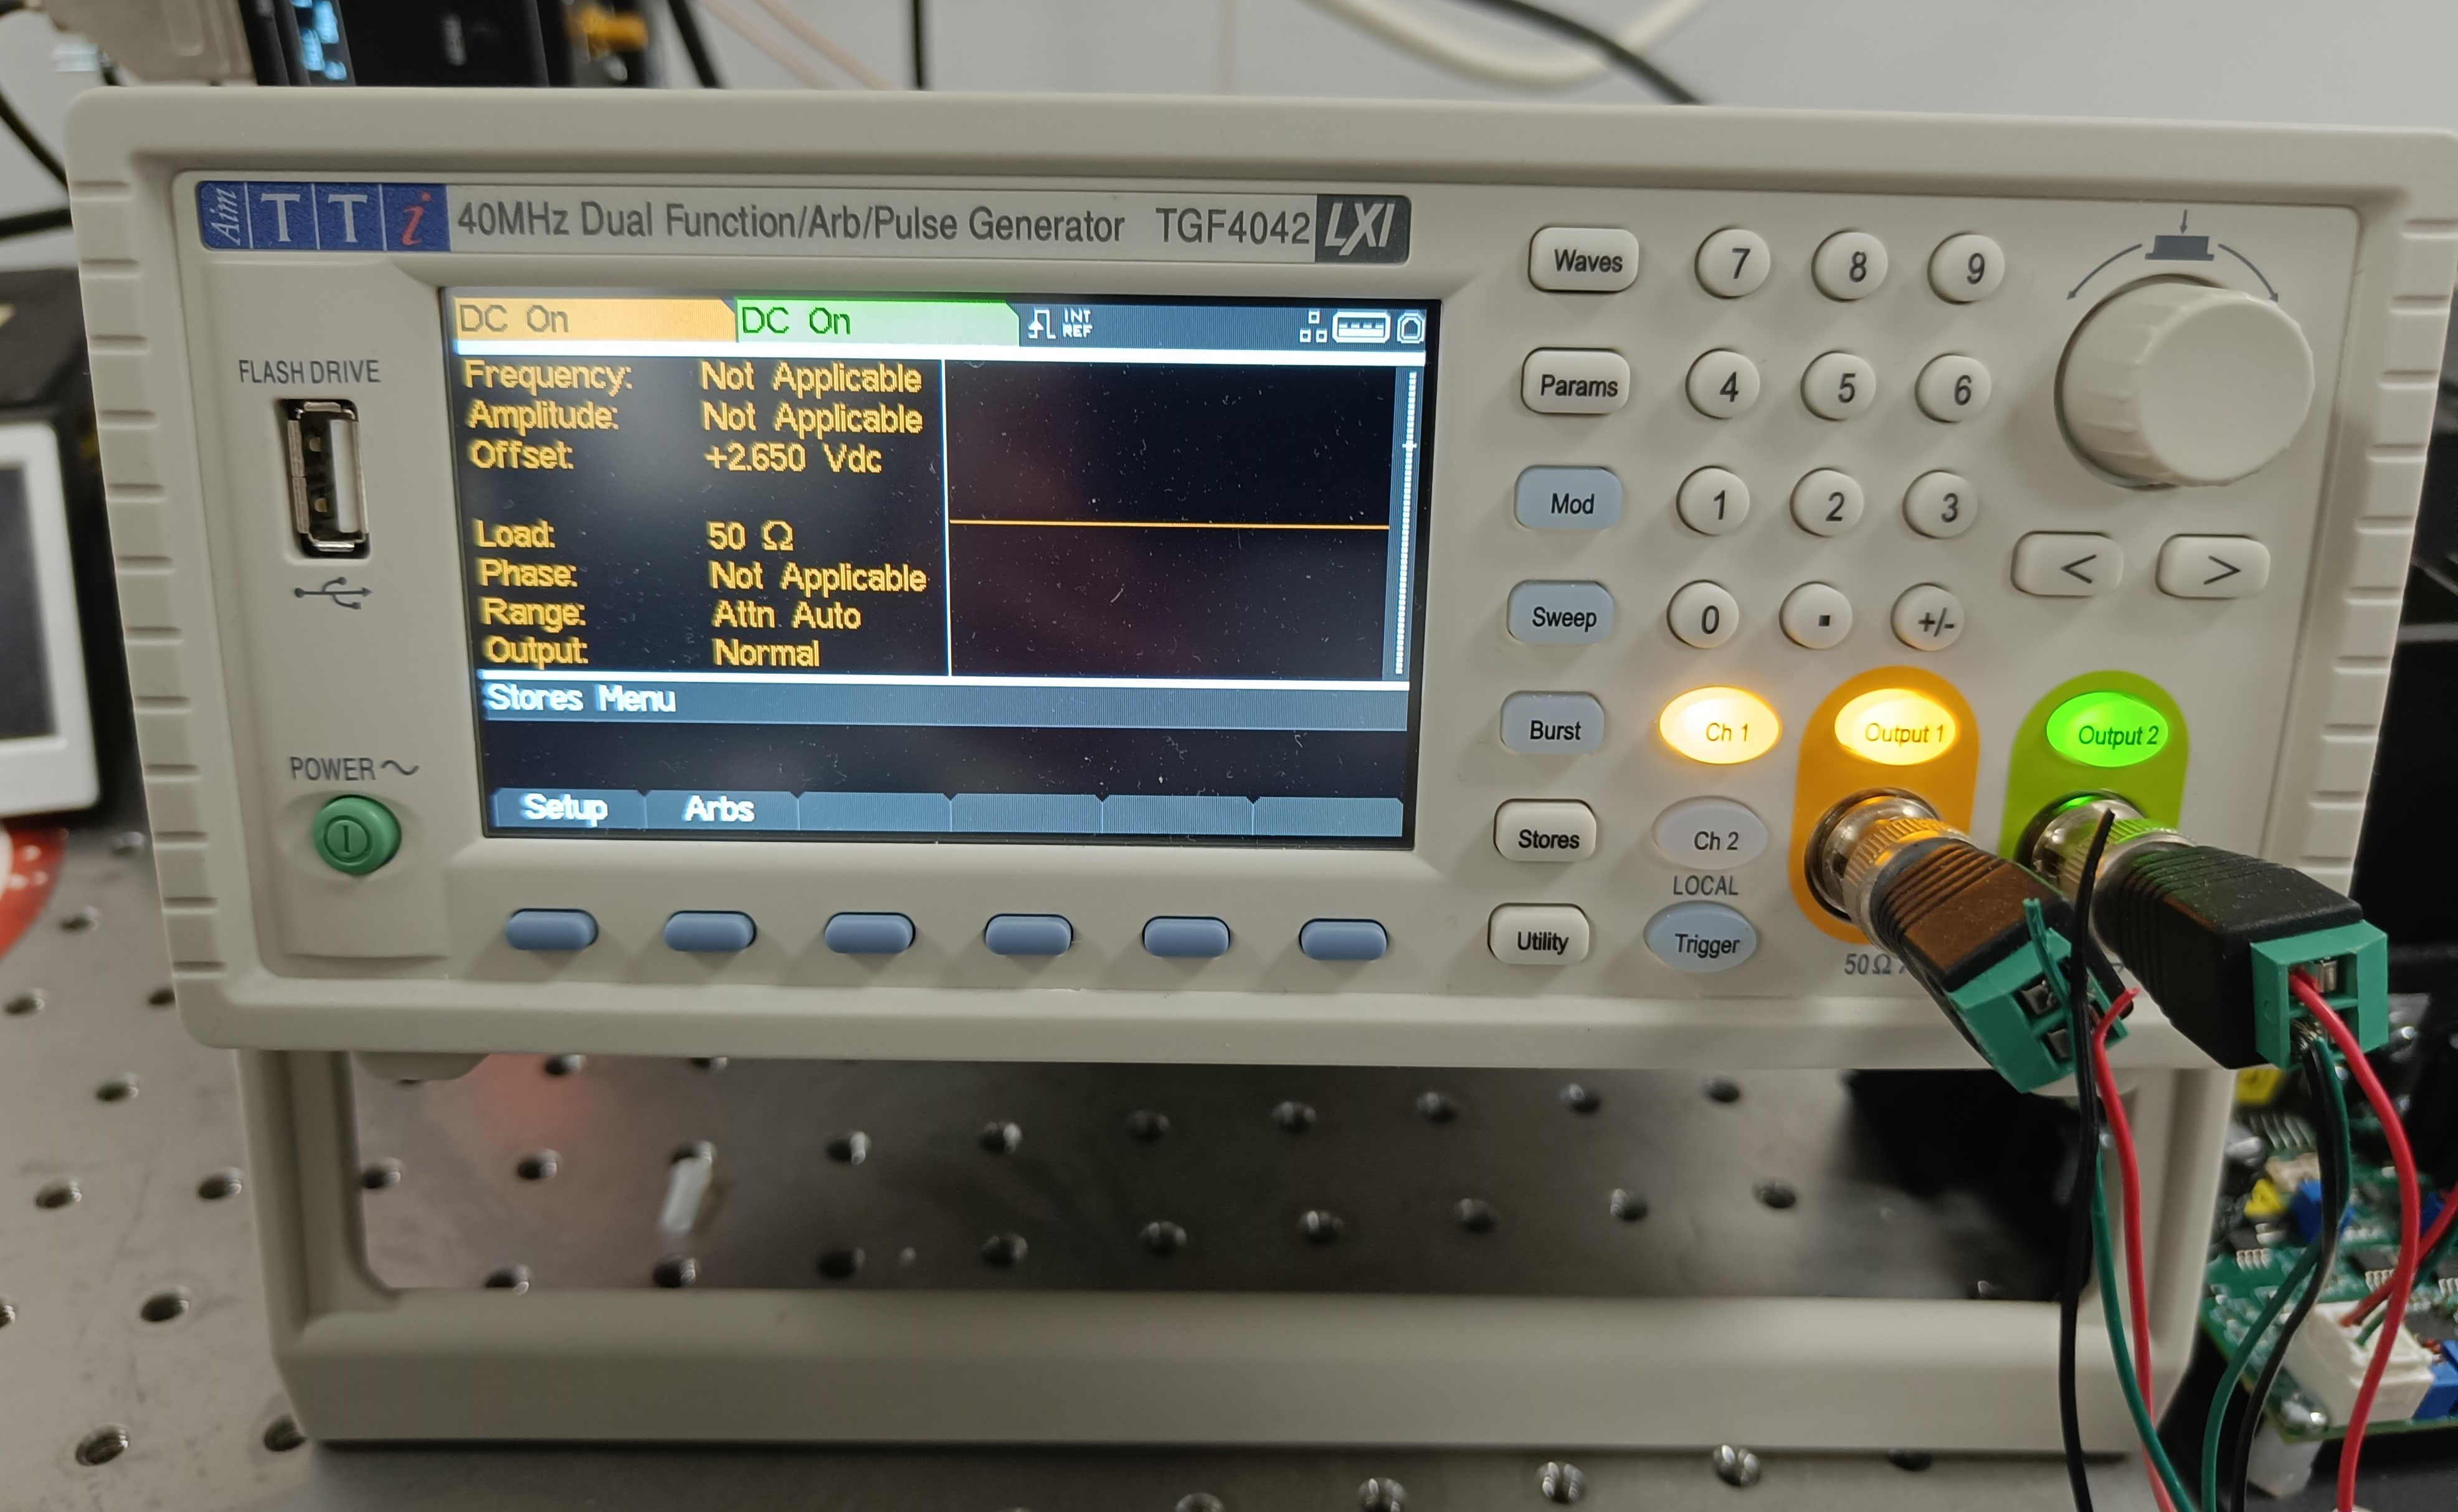
\includegraphics[width=\linewidth]{signal_generator.jpg}
		\caption{}
	\end{subfigure}
	\begin{subfigure}{0.475\linewidth}
		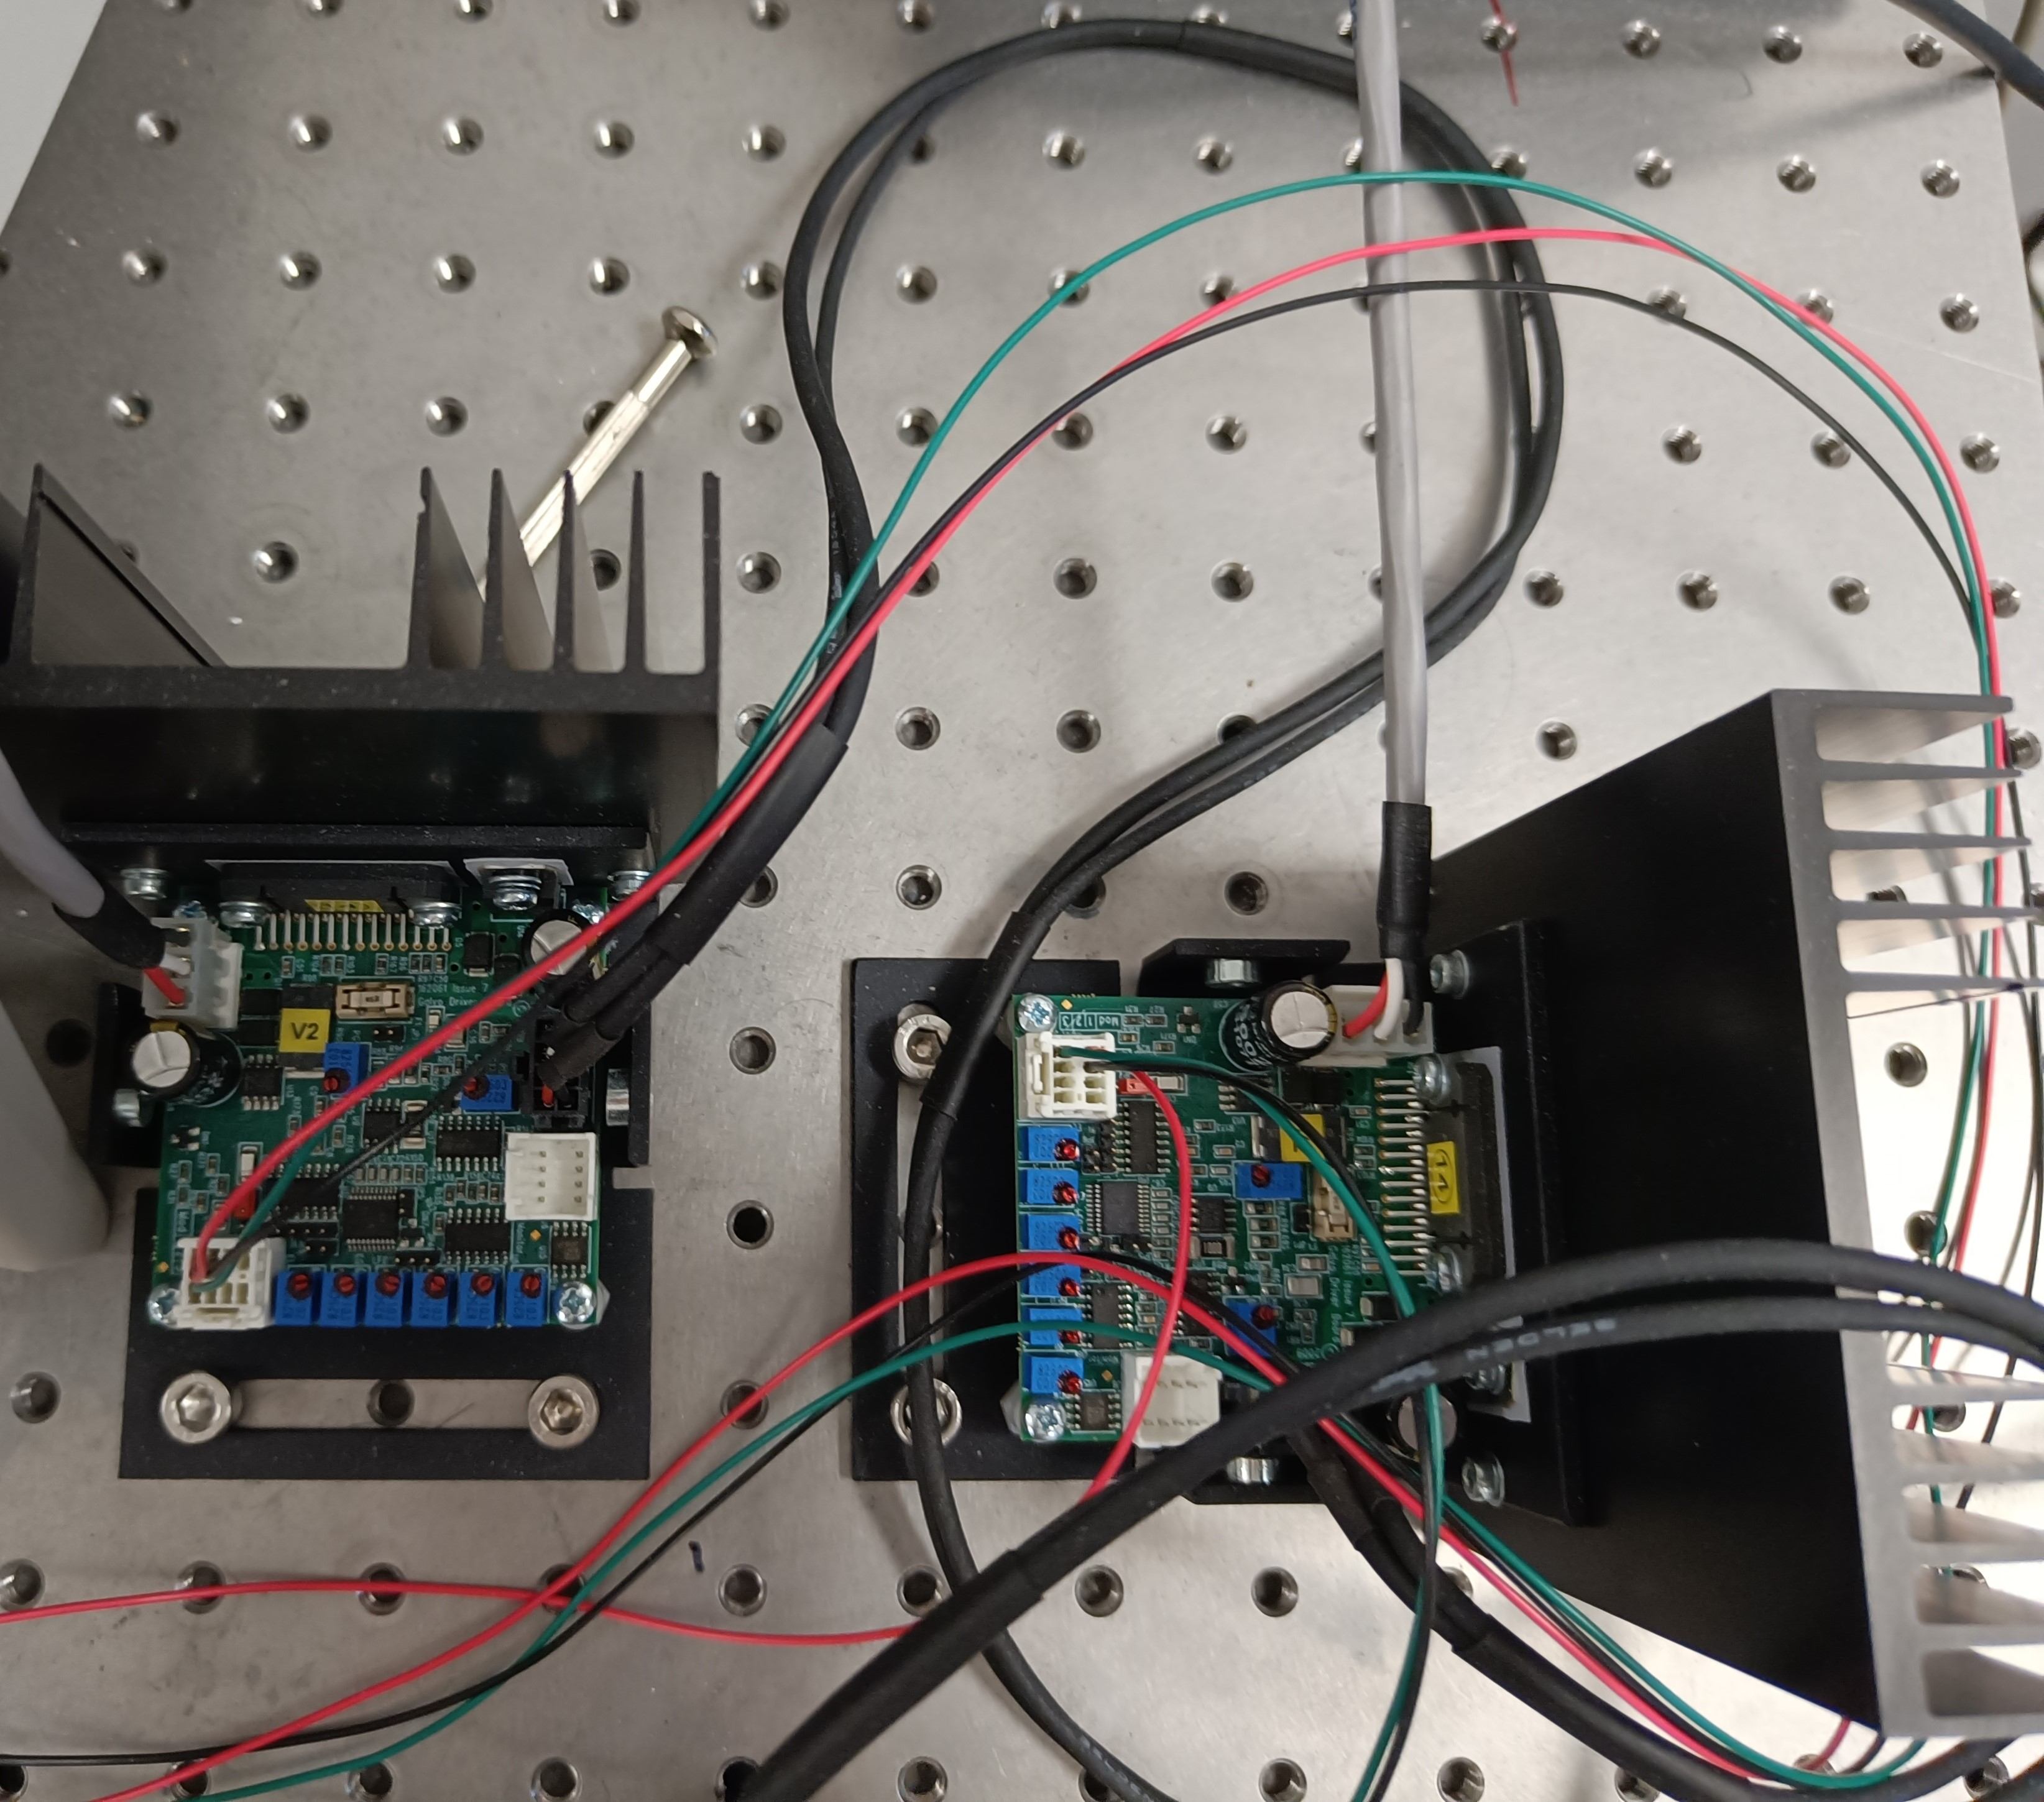
\includegraphics[width=\linewidth, height=0.7\linewidth]
		{galvano_mirror_controllers.jpg}
		\caption{}
	\end{subfigure}

	\caption{Signal generator galvano mirror controller, channel 1 controls the x-axis 
		mirror, while channel 2 controls the y-axis mirror. Both channels can be manipulated
		independently.}
\end{figure}

For our applications a 4f correlator is utilised to ensure that the motion
of the galvano-mirrors does not move the focal point of the laser, allowing 
for a stable trap even while in motion. As shown in Fig.~\ref{fig:setup}, after
the galvano-mirror we have our two lenses - $f_3$ and $f_4$ - the former being 
installed $150\ mm$ from the second mirror of the galvano, and the latter being 
installed $200\ mm$ from the back focal plane of the trapping objective. The 
signal generator used was supplied by 'MCS Test Equipment Ltd', allowing for 
dual channel signal control. This allowed us to precisely control the alignment,
amplitude, phase, and frequency of both mirrors making alignment much easier. For
basic trapping calibration the galvano-mirrors were set to a simple DC output, 
providing a fixed spot which operates like a typical optical trap.

%%%%%%%%%%%%%%%%%%%%%%%%%%%%%%%%%%%%%%%%%%%%%%%%%%%%%%%%%%%%%%%%%%%%%%%%%%%%%%%%
%%%%%%%%%%%%%%%%%%%%%%%%%%%%%%%%%%%%%%%%%%%%%%%%%%%%%%%%%%%%%%%%%%%%%%%%%%%%%%%%
\section{Synthesis of Birefringent Micro spheres}
\label{sec:vaterite}
Generation of fluid shear can be achieved via two avenues: Firstly, by 
utilising circularly polarised light it is possible to transfer angular 
momentum from the laser to the trapped entity. Secondly, one can 
directly move the trap within the imaging plane by steering the beam 
using either a galvanometric mirror or gimbal mirror. The following 
chapter outlines the work done with shear generated by circularly 
polarised light and the challenges of applying this to localising 
nucleation. 

There are several options for particles that can be rotated using 
optical tweezers \cite{Parkin2009, Saito2022}. Over the course of 
the PhD two different micro spheres where investigated, vaterite 
and liquid crystal droplets. Both can be readily synthesised in 
the lab and are will rotate at a variety of sizes. While silver 
nano particles were considered their high cost and small size 
meant they were disregarded as an option for optical rotation. 

Vaterite is a polymorph of calcium carbonate that is rarely seen in 
nature due to its low stability. However unlike its other polymorphs of 
calcite and aragonite, when synthesised vaterite will typically form 
small spherical particles making them ideal for optical trapping and rotation. 
Synthesis of vaterite micro spheres requires fine control of the nucleation
process in order to maintain polymorphic stability, though for the purposes
of optical rotation the exact polymorph is not as important as its morphology
as all 3 polymorphs are inherently birefringent. 

Vaterite samples where made by the first preparing equal amounts of 
$CaCl_2$ and $Na_2CO_3$ at a concentration of $0.33M$, at the same time
a vial of $0.33M\ MgSO_4$ was prepared and set aside for later. First
a small vial was filled with $1.5mL$ of $CaCl_2$ followed by $60\mu L$ 
and $90\mu L$ of $MgSO_4$ and $NaCO_3$ respectively, forming a seed solution. 
Next, a larger vial was filled with $5\ mL$, $1.5\ mL$, and $1\ mL$ of
$CaCL_2$, $MgSO_4$, and $NaCO_3$ respectively followed by the seed solution. 
After 10 minutes of slow but continuous mixing a few drops of Agepon was added
to halt the reaction, the solution was filtered and washed 3 times with 
distilled water before being suspended in water. When trapped in circularly 
polarised light, the anisotropic scattering of the sphere results in a periodic 
signal on the QPD. Therefore, the resulting power spectrum is not a Lorentzian
but now also displays peaks that appear at integer multiples of the particles
rotational frequency. 
\begin{figure}[h!]
	\centering
	\begin{subfigure}{0.4\linewidth}
		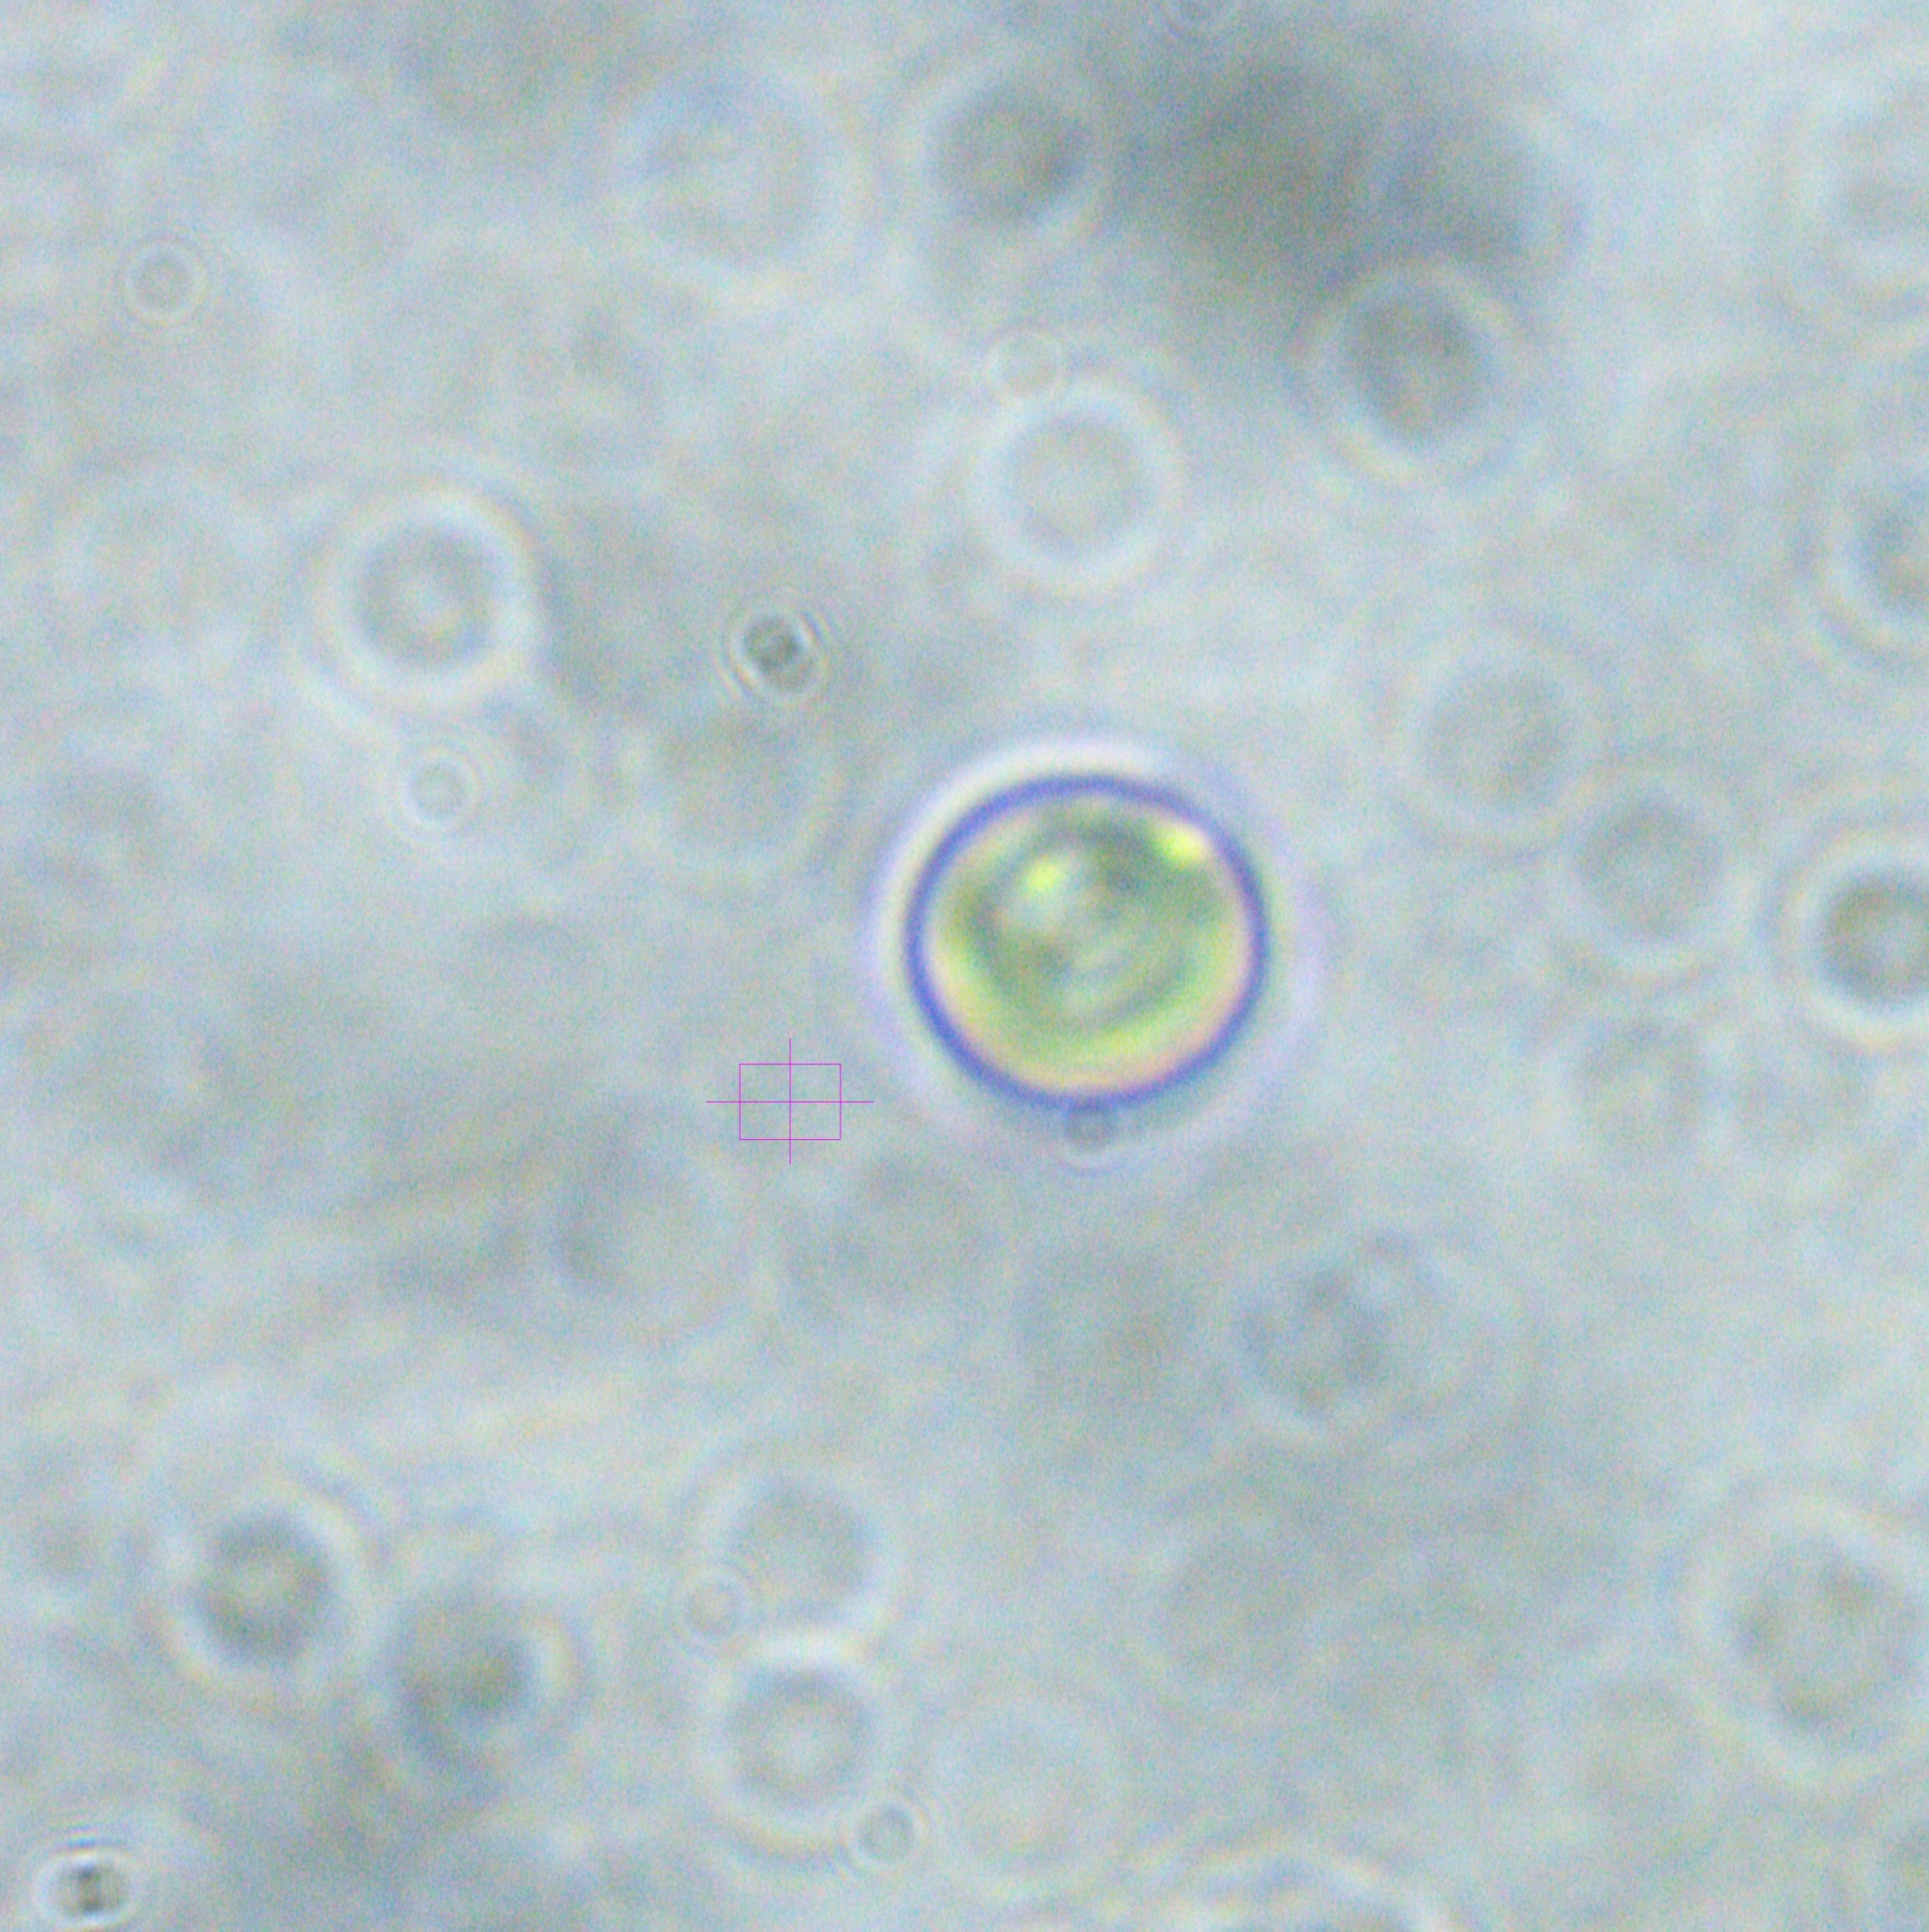
\includegraphics[width=\linewidth]{vaterite_sample.jpg}
		\subcaption{}
	\end{subfigure}
	\begin{subfigure}{0.55\linewidth}
		\includegraphics[width=\linewidth]{rotating_psd.png}
		\subcaption{}
	\end{subfigure}
	\caption{(a)Sample vaterite sphere suspended in water and trapped by circular polarised trap. (b) Collected power spectrum from rotating vaterite, peaks in the power spectrum appear at integer multiples of the rotational frequency ($f_{rot} \approx 49.8$ Hz)}
	\label{fig:vaterite}
\end{figure}

As shown by Fig.~\ref{fig:vaterite}(b) the power spectra produced still 
demonstrates a Lorentzian curve but modified with these periodic peaks, 
while the Lorentzian can be loosely fitted to the end tail there exists 
no current model for describing the power spectra. The closest approximation
to this was conducted by \cite{Yogesha2012} where they describe the 
rotational motion of ellipsoidal polystyrene particles. The critical assumption
being that the particle perfectly rotates in the $x-y$ plane; however it
has long been suspected that birefringent microspheres experience random
rotations outside of the $x-y$ plane \cite{Bang2020} making it very difficult 
to characterise the forces on rotating microspheres without a proper understanding 
of the optical torque being applied to it.

\subsection{Liquid Crystal Rotors}
Liquid crystals are an intriguing example of materials with mixed phase
properties, unlike typical solutes such as Glycine, a liquid crystal
can still maintain some degree of order between its individual molecules
while in the liquid state. This is due to the fact that liquid crystals
are constructed of long ordered molecules that demonstrate a long range
ordering. There are three main types of liquid crystal transition methods:
thermotropic crystals will transition to their liquid crystal phase when 
sufficiently heated; Lyotropic materials can undergo this transition due 
to changes in temperature and concentration; and lastly Metallotropic 
materials - which are composed of both organic and inorganic molecules - 
change phase according to the ratio of organic to inorganic molecules present.
Liquid crystal rotors are rather simple in their production, 
4-Heptyl-4-biphenylcarbonitrile (7CB) was purchased from Sigma Aldrich
and a small amount was added to a vial of distilled water. The solution 
was then heated in a water bath to $25^\circ$ in order to transition the
solid crystal into its liquid crystal state. The individual droplets 
are inherently birefringent and rotate in a circularly polarised trap. 
\begin{figure}[h!]
	\centering
	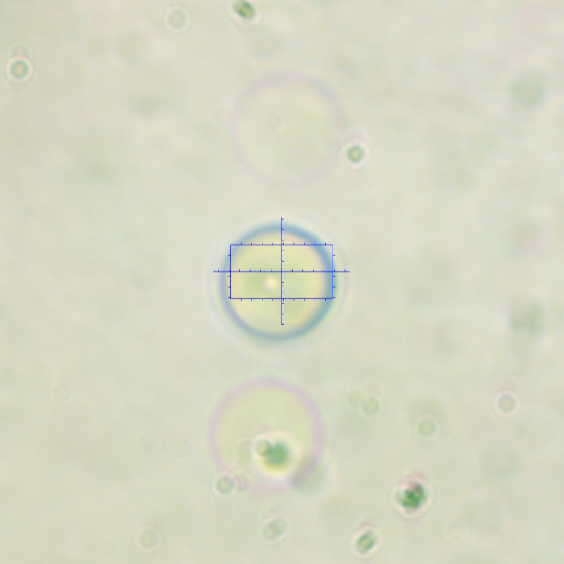
\includegraphics[width=0.5\linewidth]{LC_sample.png}
	\caption{Liquid crystal undergoing rotation due to the circularly polarised trap.} 
\end{figure}

The liquid crystal droplets had a much faster rotation rate than comparable 
vaterite spheres, due to their higher degree of birefringence and the fact
that the droplets are far closer to perfect spheres making angular momentum
transfer more efficient. 

%%%%%%%%%%%%%%%%%%%%%%%%%%%%%%%%%%%%%%%%%%%%%%%%%%%%%%%%%%%%%%%%%%%%%%%%%%%%%%%%
\subsection{Rotation of birefringent micro spheres} 
Optical tweezing has often been used for micro-rheology, by computing the
exact forces being exerted on the trapped sphere, one can determine the
local temperature/viscosity of the medium \cite{Millen2014, RodriguezSevilla2018}.
Using a birefringent particle and rotating it within the fluid, the maximum 
rotation rate is due to the fluid drag resisting the torque of the 
trapping beam \cite{RodriguezSevilla2018}. If you want to measure 
fluid flow you can instead use a micro-rotor to see how fluid flow 
propagates in the medium \cite{Knoener2005}. Likewise, one can use 
a galvanometric mirror to probe the drag force of the fluid, by 
understanding the trap strength (calibrating using a low frequency 
signal) one can measure the drag force experienced by the local fluid \cite{RobertsonAnderson2018}. I

Understanding the fluid velocity around our trapped object is determined 
mostly by the Reynold's number of our system, for a sphere submersed 
in a moving fluid of velocity $U$ this is given by:
\begin{align}
	Re = \frac{\rho UD}{\mu}
\end{align}

Where $D$ is the sphere's diameter, and $\rho$ and $\mu$ are the fluid's 
density and viscosity respectively. In our case we do not have a fluid
moving around a sphere but a sphere moving through the fluid at some 
velocity $U$, assuming a no-slip boundary condition we can model the 
fluid velocity profile based on the velocity of the particle. There are 
two possible avenues for generating shear flow with a trapped particle; 
rotation of birefringent particles, and fluid flow induced by particle motion. 

Rotating birefringent particles are by far the most common method for 
generating and measuring fluid flow in a solution. To see if we can 
even achieve the theoretical maximum shear rate, vaterite spheres 
were synthesised (see Sec.\ref{sec:vaterite}) submerged in water and 
trapped with the 1064 nm laser at set to 450 mW. The rotation frequency 
was determined using the QPD, and the particle sizes were computed 
by image analysis. With the particle size and rotation frequency, the 
tangential rotation speed is calculated via:
\begin{align}
	\label{eq:birefringent_speed}
	u(r) = \frac{\pi}{4}\frac{d^3}{r^2}\omega
\end{align}

Where $d$ is the particle diameter, $\omega$ is the rotation frequency
reported by the QPD, and $r$ is the distance from the particle's centre. 
Using Eq.\ref{eq:birefringent_speed} we computed the fluid flow radiating
outward from the centre of the sphere. The shear rate can then be computed
as the partial derivative fluid flow (assuming shearing is generated purely
by the flow field):
\begin{align}
	\label{eq:birefringent_shear}
	\dot{\gamma}(r)=\left|\frac{\delta u(r)}{\delta r} \right|= \frac{\pi}{2}\frac{d^3}{r^3}\omega
\end{align}

First we tested the rotational behaviour of vaterite in distilled water, 
samples of vaterite where diluted down and $200\mu L$ was pipetted onto
the sample stage. Due to Van der Waal's forces some of the microspheres 
were stuck together, fortunately individual sphere's were still present.
Over the course of a few weeks multiple sphere's where trapped 
and their rotation speeds were measured via the QPD. 
\begin{figure}[h!]
	\begin{subfigure}{0.5\linewidth}
		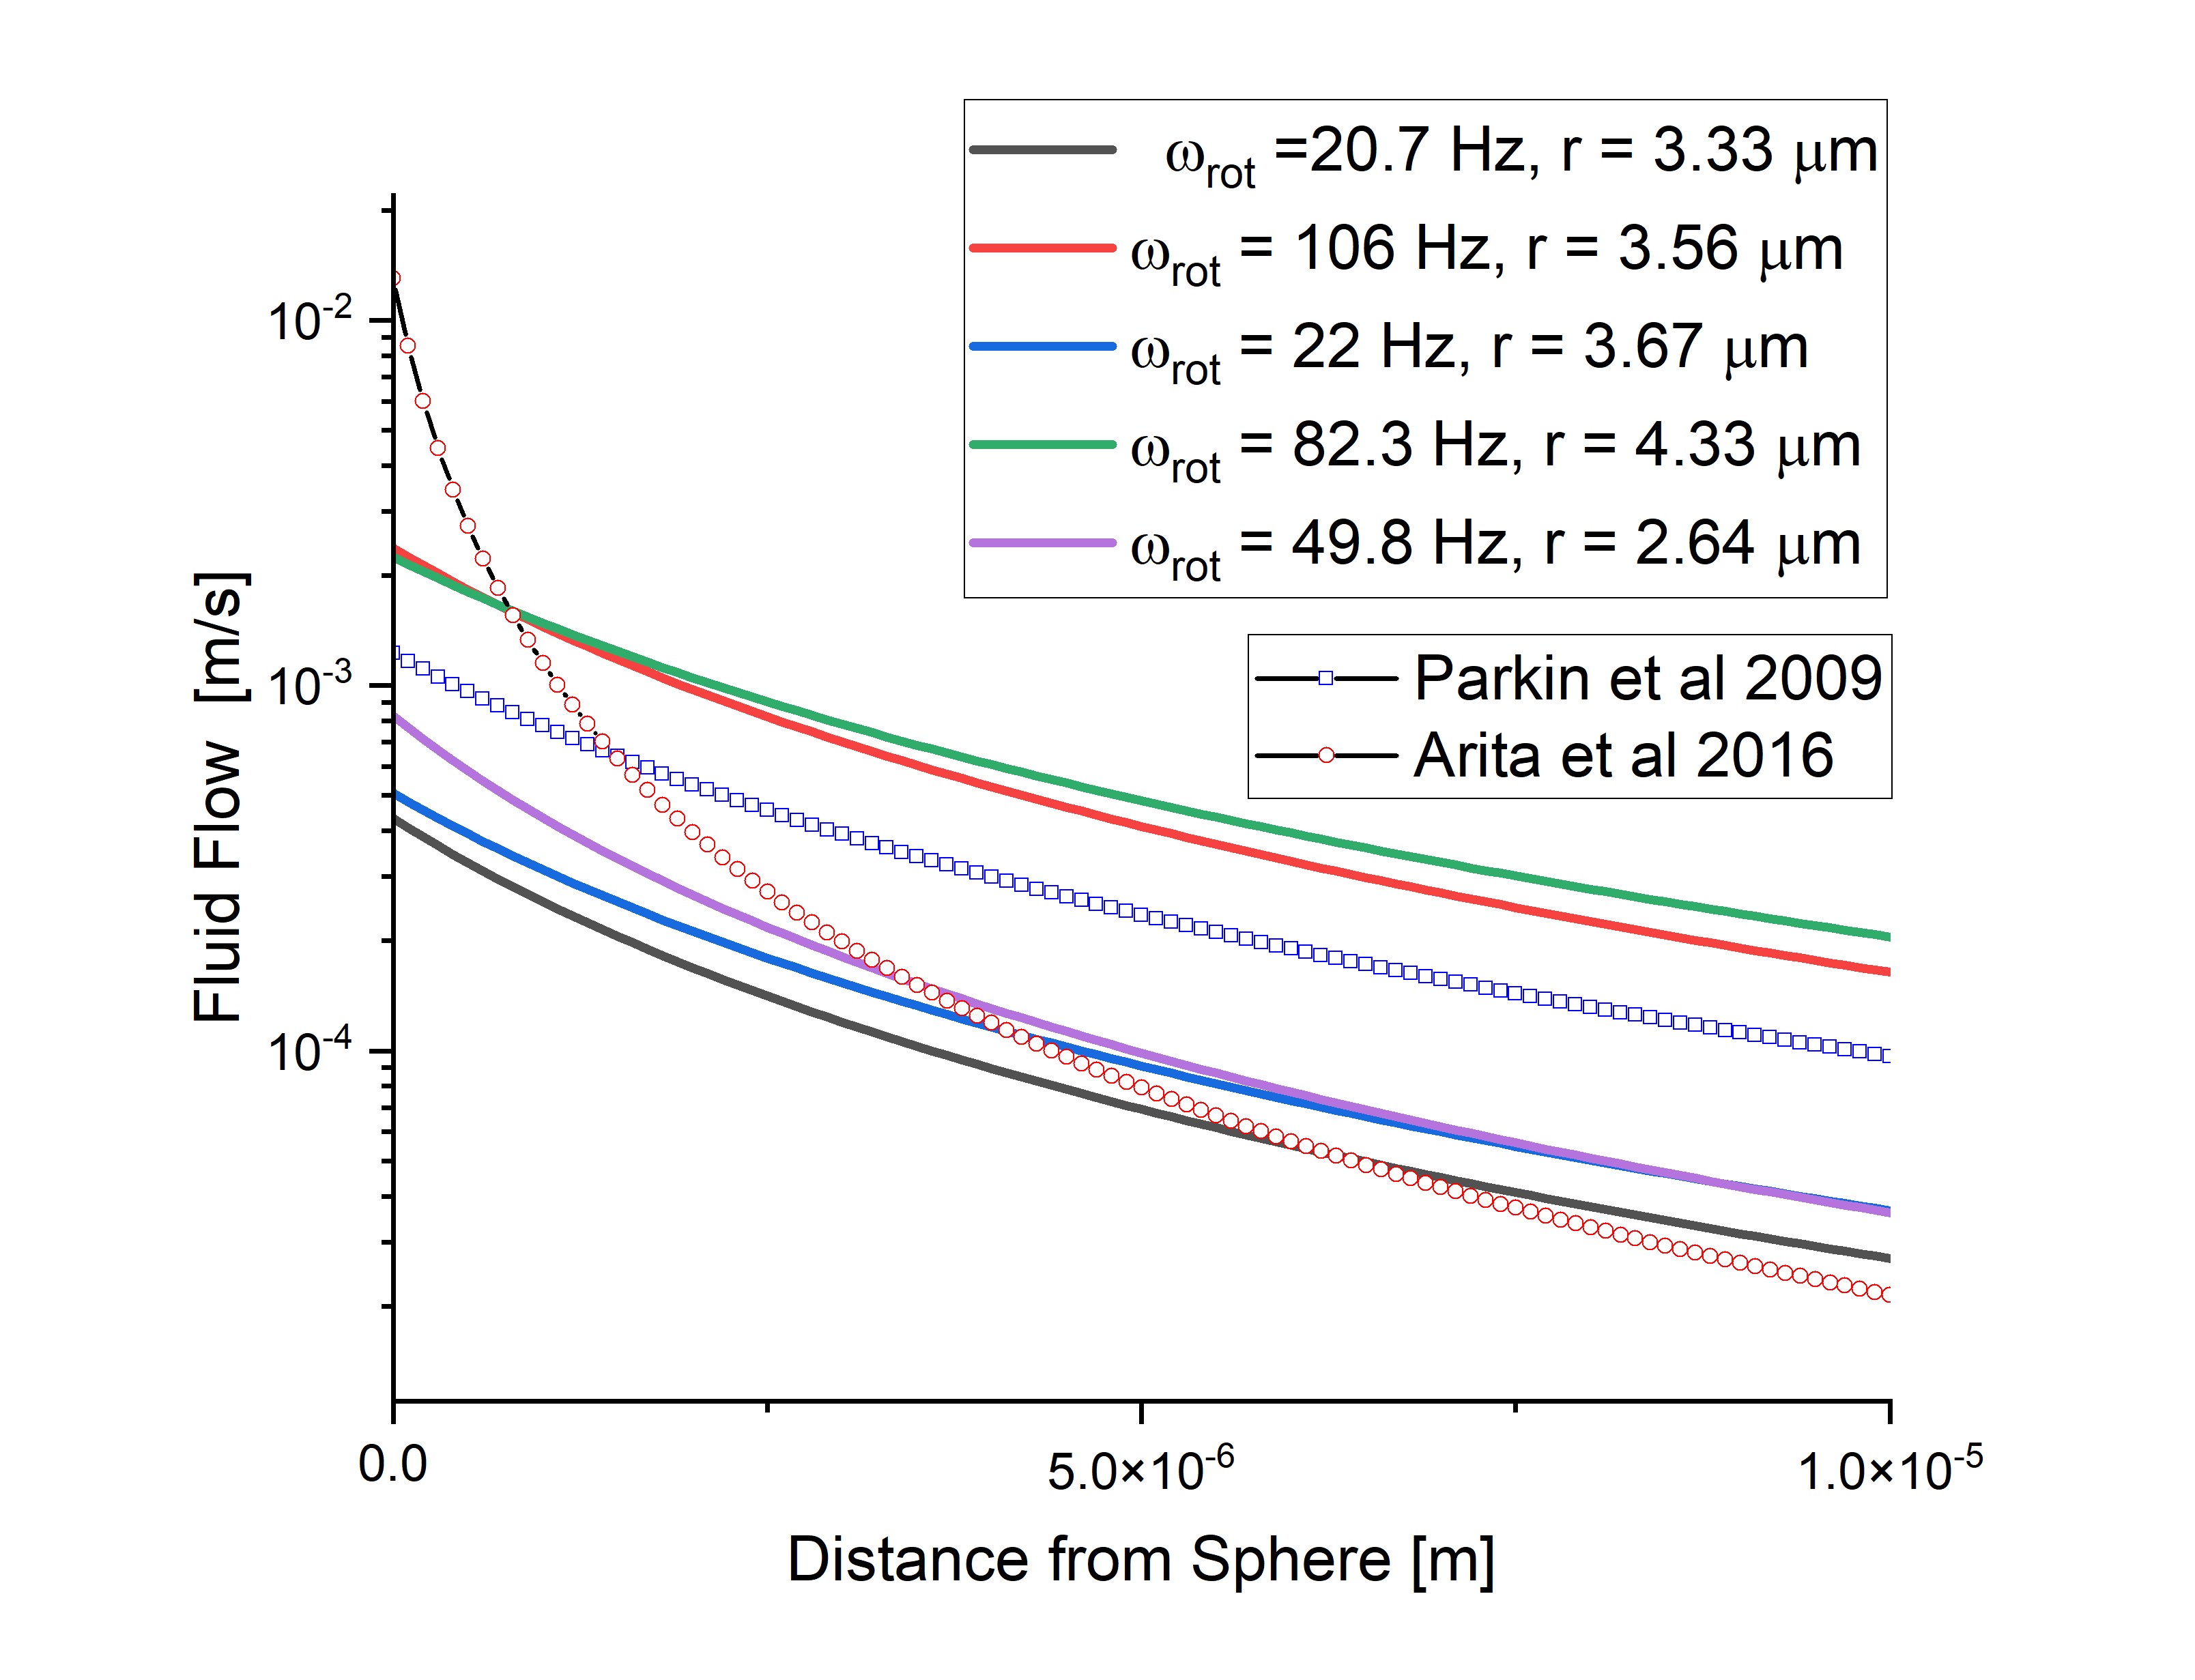
\includegraphics[width=\linewidth]{vaterite_fluid_flow.png}
		\subcaption{}
	\end{subfigure}
	\begin{subfigure}{0.5\linewidth}
		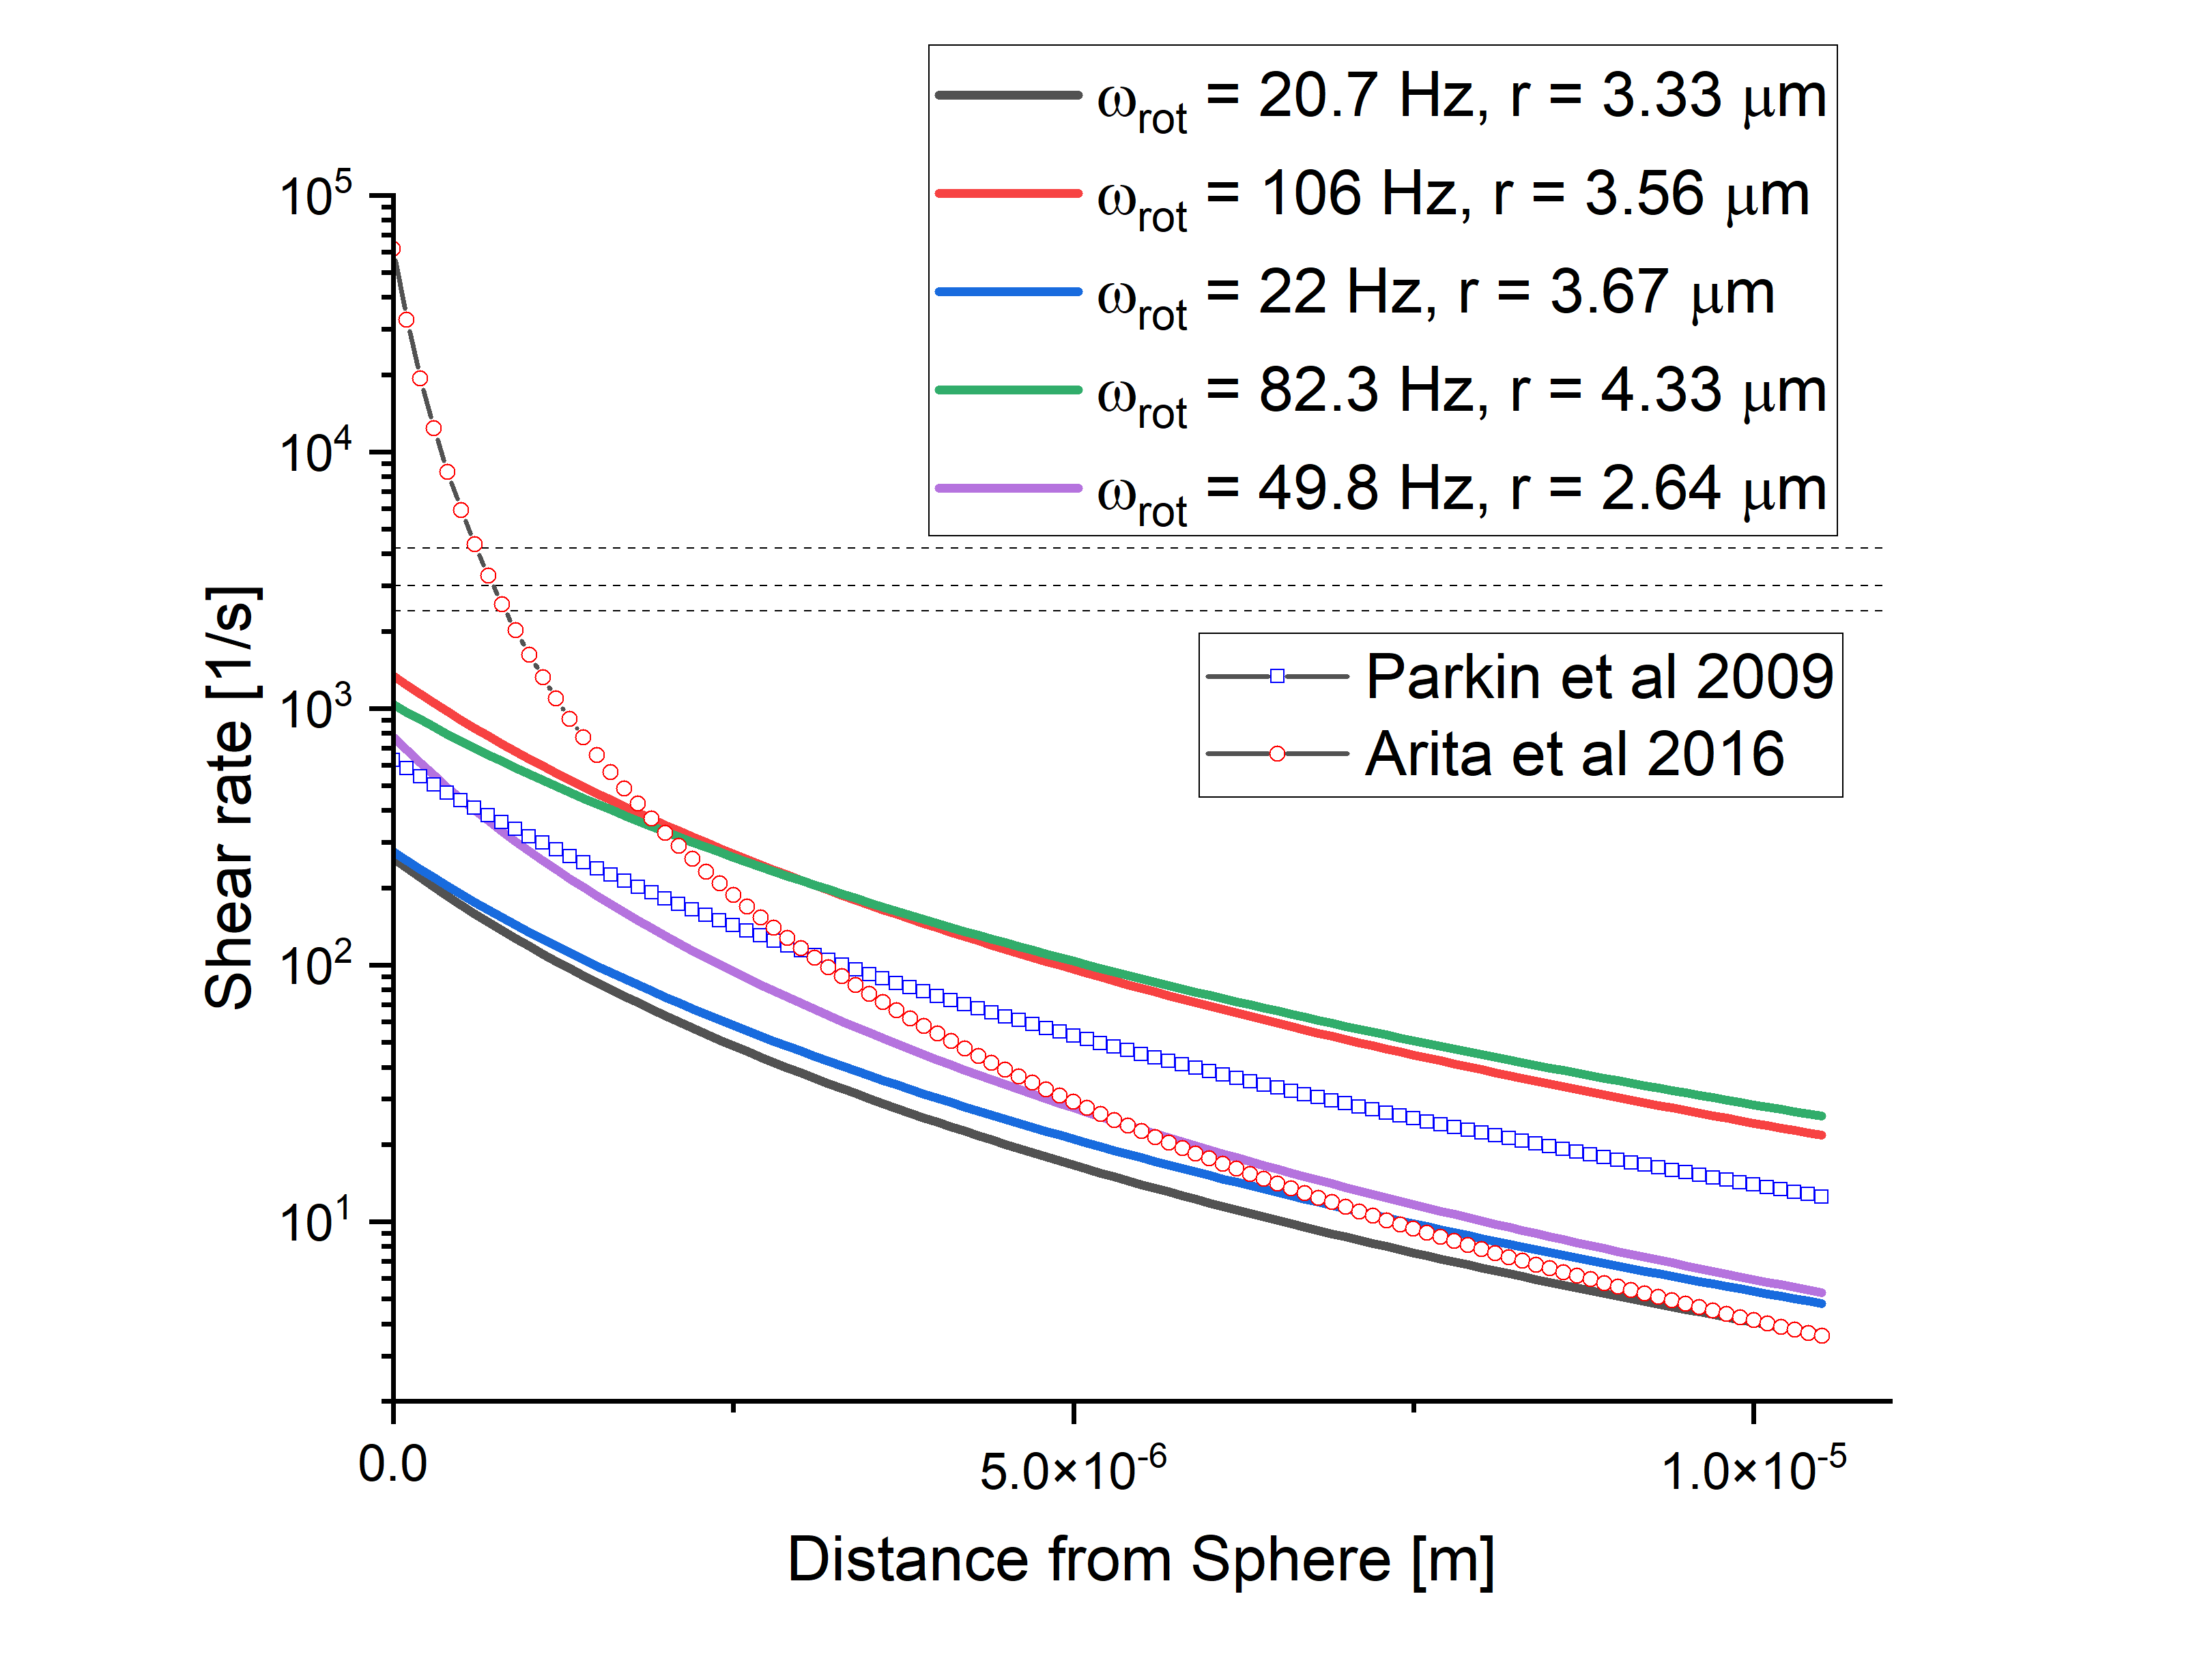
\includegraphics[width=\linewidth]{vaterite_shear_rate.png}
		\subcaption{}
	\end{subfigure}
	\caption{(a) Fluid flow radiating out from the surface of a rotating vaterite sphere. (b) Shear rates computed using Eq.\ref{eq:birefringent_shear}, optimal shear rate is of $3000 s^{-1}$ is indicated by the dotted line. Vaterite radii and rotation frequencies are shown, the laser power was kept constant at 450 mW. Reported rotation rates, and their corresponding fluid flow and shear rates, for vaterite are also plotted alongside lab results.}
	\label{fig:vaterite_shear}
\end{figure}

From Fig.\ref{fig:vaterite_shear} there is not a strong relationship between
particle size and rotation rate, this is contrary to much of the theoretical
predictions that predict an exponential decay with particle size. This can
be in part due to the fact that synthesising perfectly spherical spheres that
have uniform birefringence is difficult over multiple experiments and tests. 
Despite our best efforts at controlling the growth rate the vaterite spheres
would often combine together while suspended in water after a short period of 
time. The fastest reported rotation rate found during this PhD was by \cite{Arita2016}
that achieved a rotation rate of $5\ kHz$, this is plotted on Fig~\ref{fig:vaterite_shear}
as the dotted line. Even at that extreme a rotation rate the region in which 
nucleation is at its optimal likelihood is only $20\ nm$ wide meaning that 
localising nucleation around a rotating sphere is vanishingly small. 

%%%%%%%%%%%%%%%%%%%%%%%%%%%%%%%%%%%%%%%%%%%%%%%%%%%%%%%%%%%%%%%%%%%%%%%%%%%%%%%%
%%%%%%%%%%%%%%%%%%%%%%%%%%%%%%%%%%%%%%%%%%%%%%%%%%%%%%%%%%%%%%%%%%%%%%%%%%%%%%%%
\section{Rotation of micro-rotors in supersaturated solutions}
Vaterite samples were synthesised according to \cite{Parkin2009, Bishop2004} 
(see sec.~\ref{sec:vaterite}), and then suspended in distilled 
water, at the same time a supersaturated solution of Glycine 
and water was prepared and $50\ \mu L$ was pipetted onto a 
glass cover slip. A single microsphere the vaterite was trapped 
in a circularly polarised light and brought close to the droplet 
edge.
\begin{figure}[h!]
	\centering
	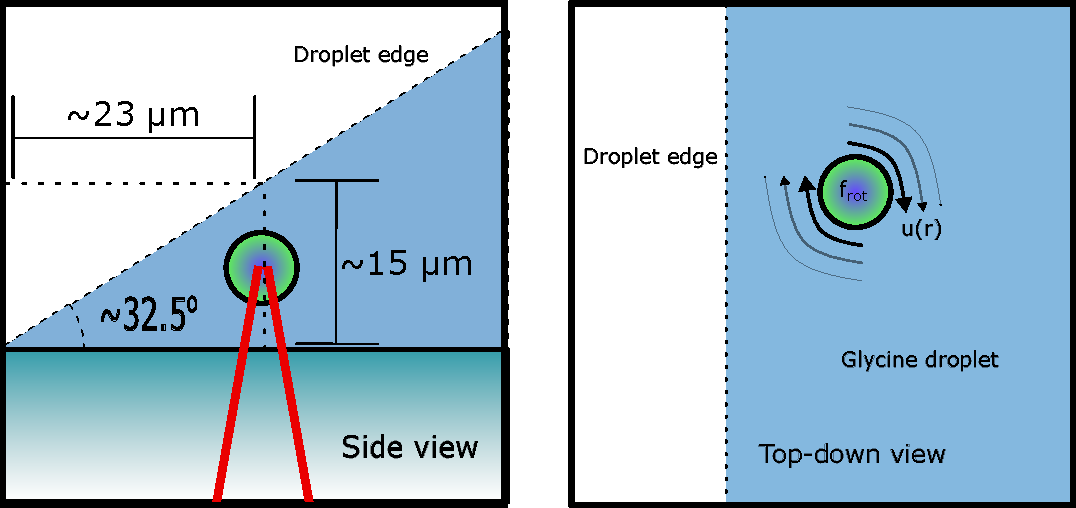
\includegraphics[width=\linewidth]{vaterite_diagram.pdf}
	\caption{Diagram of optical trapping set up for rotating birefringent 
		particles in a supersaturated solution. Left: side view of the 
		trapping set up showing the location of the trap focus at the 
		edge of the droplet of a supersaturated solution. Right: top down 
		view of the glycine droplet with a trapped birefringent particle 
		shown close to edge of the trap. As the particle rotates the drag 
		force from the surrounding fluid generates a flow field around 
		itself (see Eq.~\ref{eq:birefringent_speed}).}
\end{figure}

After a period of ten minutes if no nucleation event was 
observed the particle was released and another particle was 
trapped. Due to the increased viscosity of the supersaturated 
solution and the proximity to the droplet edge, as previous works
have only seen nucleation near the solution-air interface \cite{Gowayed2021, 
Liao2022, Walton2018}, the observed rotation rate was rather low or 
non-existent, the results are tabulated below:
\begin{table}[h!]
	\centering
	\caption{Results from rotating vaterite within supersaturated solution of $H_2O$ and Glycine. Solubility concentration for Glycine at $16^\circ$ was $C^*=0.2016g/g$}
	\begin{tabular}[width=\textwidth]{|c|c|c|c|}
		\hline
		Super Saturation & Particle radius [$\mu$] & $\omega$ [Hz] & Nucleation [$\checkmark/\times$]\\
		\hline
		\multirow{3}*{1.01} & 2.34 & 20.7 & $\times$ \\
		\cline{2-4} & 5.67 & 23.3 & $\times$ \\
		\cline{2-4} & 3.26 & 15.4 & $\times$ \\
		\hline
		\multirow{3}*{1.14} & 1.89 & 1.23 & $\times$ \\
		\cline{2-4} & 3.75 & 3.54 & $\times$ \\
		\cline{2-4} & 4.35 & 4.86 & $\times$ \\
		\hline
		\multirow{3}*{1.4} & 3.47 & 0.00 & $\times$ \\
		\cline{2-4} & 1.59 & 0.00 & $\times$ \\
		\cline{2-4} & 6.24 & 0.00 & $\times$ \\
		\hline
		\multirow{3}*{1.45} & 6.32 & 0.00 & $\times$ \\
		\cline{2-4} & 3.68 & 0.00 & $\times$ \\
		\cline{2-4} & 5.43 & 0.00 & $\times$ \\
		\hline
		\multirow{3}*{1.49} & 4.76 & $0.00$ & $\times$ \\
		\cline{2-4} & 7.27 & $0.00$ & $\times$ \\
		\cline{2-4} & 1.52 & $0.00$ & $\times$ \\
		\hline
	\end{tabular}
\end{table}

The calculations from fig.\ref{fig:vaterite_shear} indicate that even
in pure water the rotational speed achieved by a microsphere is
insufficient to achieve a significant shear rate more than a few tenths of a microns
from its surface. The closest we could trap a microsphere to the droplet
edge was in the range of $5-10\mu\ m$, at that distance the fluid flow
would be so low that not even using a liquid droplet rotor would achieve
the rotational speeds necessary to localise nucleation. While in theory
a sufficiently focused laser could rotate any microsphere to a fast enough 
to match the speeds expected by \cite{Debuysschere2023} the localised intensity
would be so large that even using $D_2O$ would see a significant increase in 
temperature. 

It is not impossible that fluid shearing could be used in the future to localise
nucleation; but from these results, using individual micro-rotors do not seem like 
an appropriate method. If multiple micro-rotors could be trapped in close proximity 
to one another they could create a large region of fluid where nucleation is more 
likely than the bulk fluid. Micro-rotors have been created that allow for precise
control of suspended micro-particles \cite{Butaite2019} and could potentially be
used to generate sufficient shearing, however these could not be used in this PhD 
as we lacked the necessary hardware to form multiple gradient traps.  


%%%%%%%%%%%%%%%%%%%%%%%%%%%%%%%%%%%%%%%%%%%%%%%%%%%%%%%%%%%%%%%%%%%%%%%%%%%%%%%%
%%%%%%%%%%%%%%%%%%%%%%%%%%%%%%%%%%%%%%%%%%%%%%%%%%%%%%%%%%%%%%%%%%%%%%%%%%%%%%%%
\section{Shearing via a Galvano-mirror}
Rather than utilising birefringence rotation, which is subject to issues
during synthesis and achieving an ideal particle size, a galvano-mirror
was installed to induce controlled particle motion. While typically 
galvano and gimble mirrors are used to trap multiple particles in a 
regular pattern, in a sufficiently dilute solution a single silica 
micro sphere can be moved quickly through a fluid along a preset path.
Calculating the shear rate around an individual particle is difficult to
do precisely but for low Reynolds numbers we can get an adequate approximation.

For a simple circular path one can estimate the sphere's speed by the 
radius of its path and the frequency of its orbit $U = R\omega$; however 
for a more complex path, such as an elliptical orbit the curve needs 
to be parametrised. One can describe the position parameter of a circular 
path as such:

\begin{align}
	r(u) = \left[rcos(2\pi u), rsin(2\pi u), 0 \right]
\end{align}

If we say that $u$ describes time from some initial point we can say $u=t\omega$ 
where omega is the frequency of orbit. Substituting this in and then taking 
the partial derivative of position gives:

\begin{align}
	v(t) = \frac{dr(t)}{dt} = \left[-2\pi r\omega \ sin(2\pi t\omega),
	\ 2\pi r\omega \ cos(2\pi t\omega), 0 \right]
\end{align}

In order to compute U we simply take the magnitude of our velocity. 
For low velocities the fluid flow at the sphere's surface can be computed 
based on its velocity.

\begin{align}
	u_r(r)=-|v(t)|^2cos(\theta)\left(1-\frac{3R}{2r}+\frac{R^3}{2r^3}\right)
\end{align}

Where $\theta$ is the angle from the direction of movement to the point
you wish to measure, and $r$ is the radial distance to that point. Again
taking the partial derivative we can get the shear rate for a particle moving 
through the fluid:

\begin{align}
	\dot{\gamma}(r) = \left| \frac{\delta u_r(r)}{\delta r}\right| = |v(t)|^2cos(\theta)\left(\frac{3R}{r^2} -\frac{2R^3}{r^4} \right)
\end{align}

Moving a silica bead along an circular path can generate significant fluid 
flow around a larger volume compared to comparable microspheres.

%%%%%%%%%%%%%%%%%%%%%%%%%%%%%%%%%%%%%%%%%%%%%%%%%%%%%%%%%%%%%%%%%%%%%%%%%%%%%%%%
%%%%%%%%%%%%%%%%%%%%%%%%%%%%%%%%%%%%%%%%%%%%%%%%%%%%%%%%%%%%%%%%%%%%%%%%%%%%%%%%
\section{Nucleation using a moving beam}
As mentioned previously, shearing via optical rotation and particle displacement
did not result in any localised nucleation events even while in the proximity of 
the droplet edge. During the experiments with the galvano-mirror, it was found 
that when no particle was present in the optical trap nucleation events would 
occur while the beam was close to the edge of the droplet, even though the solution
was undersaturated. This has been reported prior \cite{Rungsimanon2010, Liao2022}, 
but was more interesting is how the beam's motion influenced the growth of the nucleus.

Consider below in Fig.~\ref{fig:stationary_beam} the frames taken from a nucleation 
event in supersaturated glycine solution ($S=1.03$), the beam is a stationary being 
$\approx3.5 \mu m$ from the droplet edge. After a period of roughly 5 minutes a 
nucleus forms at the trap focus, growing quickly (growth rate was approximated using
imageJ to be on the order of $700\ \mu m^2/min$) from the focal point of the trap 
until after roughly $6$ seconds the crystal escapes. Comparing to previous literature
using optical tweezers shows that the growth rate is only loosely connected to the 
solutions supersaturation, local conditions play a much larger role in the growth 
rate than just the concentration \cite{Flannigan2023}. A likely reason that the trap 
is escaped is due to the fact that crystal is far too large to be held in place and 
is in fact still growing as the solution is supersaturated. The key take away to 
remember is that the beam has no real influence over the crystal shape, instead 
it grows outward from the trap focus.
\begin{figure}[h!]
	\centering
	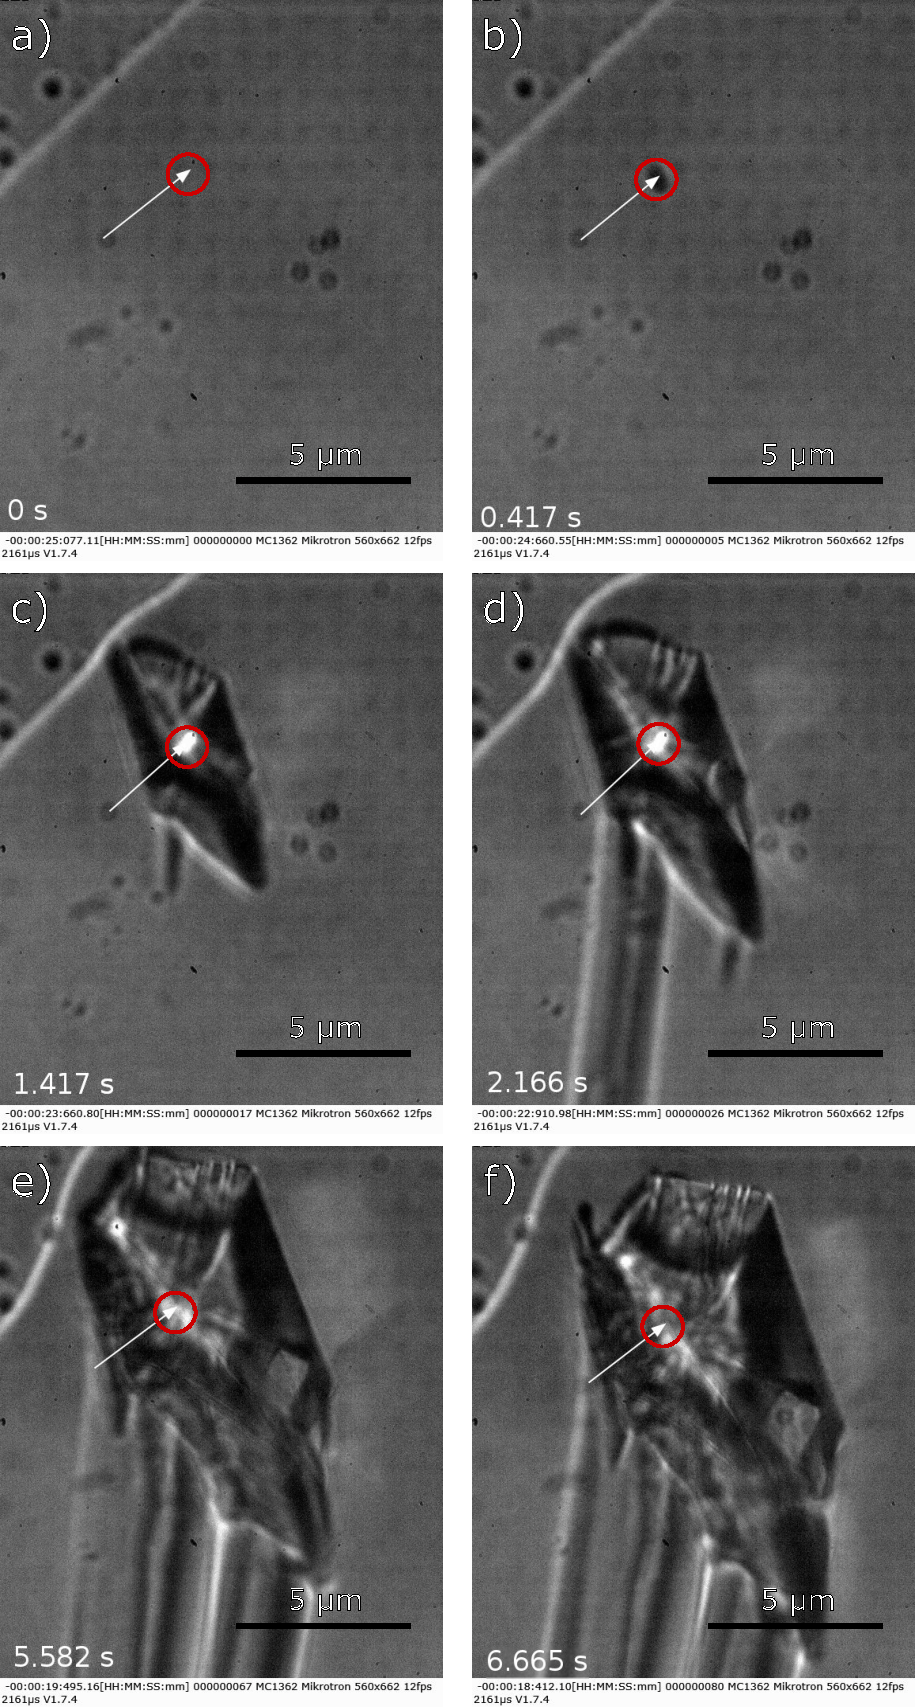
\includegraphics[width=0.7\linewidth]{frames_no_beam_movement.pdf}
	\caption{Laser induced nucleation at the edge of a droplet of supersaturated 
	glycine solution. (b) shows the first instance of a crystal nucleus, growing 
	quickly through (c)-(e) until after $6.665\ s$ the crystal begins to escape the trap.}
	\label{fig:stationary_beam}
\end{figure}

Now while trying to induce fluid flow by optically trapping a silica particle and 
using a galvano-mirror to move the particle through the solution, nucleation events
were observed in which crystal growth follows the laser focus. Shown below in Fig.~\ref{fig:eliptical_beam_1} where we have the laser focus moving in a small elliptical 
pattern; interestingly, due to the addition of the silica suspension we see the presence
of small spheres, these appear too small to be silica beads which have a uniform radius
of $1.57\ \mu m$, we surmise these could be small clusters of Glycine that had previously
been shown to form when the aqueous solutions where irradiated with a focused laser
\cite{Tsuboi2009, Gowayed2021}. While no droplets are seen directly entering the focus a 
nucleus forms close to the droplet edge, unlike in Fig.~\ref{fig:stationary_beam} the 
crystal does not grow out from the focal point evenly; due to the galvano mirror, 
the crystal is simultaneously being moved by and growing around the focal point of 
the trap. Because of this the crystal nucleus lacks a clear morphology at first, 
until roughly $20\ s$ the crystal reaches a almost prismatic structure, with further 
irradiation increasing the size. Interestingly the galvano-mirror allows the trap to 
impart a slight torque on the crystal, as shown in fig.~\ref{fig:eliptical_beam_1}(c) 
and (d), where even though the crystal is not directly in the trap focus it rotates in 
the $x-y$ plane and gets trapped again at a corner. The rotation could not be due to fluid
flow close to the surface of the crystal as trap should have no influence on fluid molecules
smaller than a few hundred nano-meters. In figs.\ref{fig:eliptical_beam_1}(e) and (f), 
the crystal growth is localised to the corner, even though previously the crystal growth 
was roughly uniform (compare figs. \ref{fig:eliptical_beam_1}(b) and (c)). The area growth
rate between figures \ref{fig:eliptical_beam_1}(a) and (d) was approximated using imageJ at
$45.03\ \mu m^2 /min$, where as between figures \ref{fig:eliptical_beam_1}(e) and (f) the 
growth rate at that particular edge was estimated at $42.10\ \mu m^2/min$. 
\begin{figure}[h!]
	\centering
	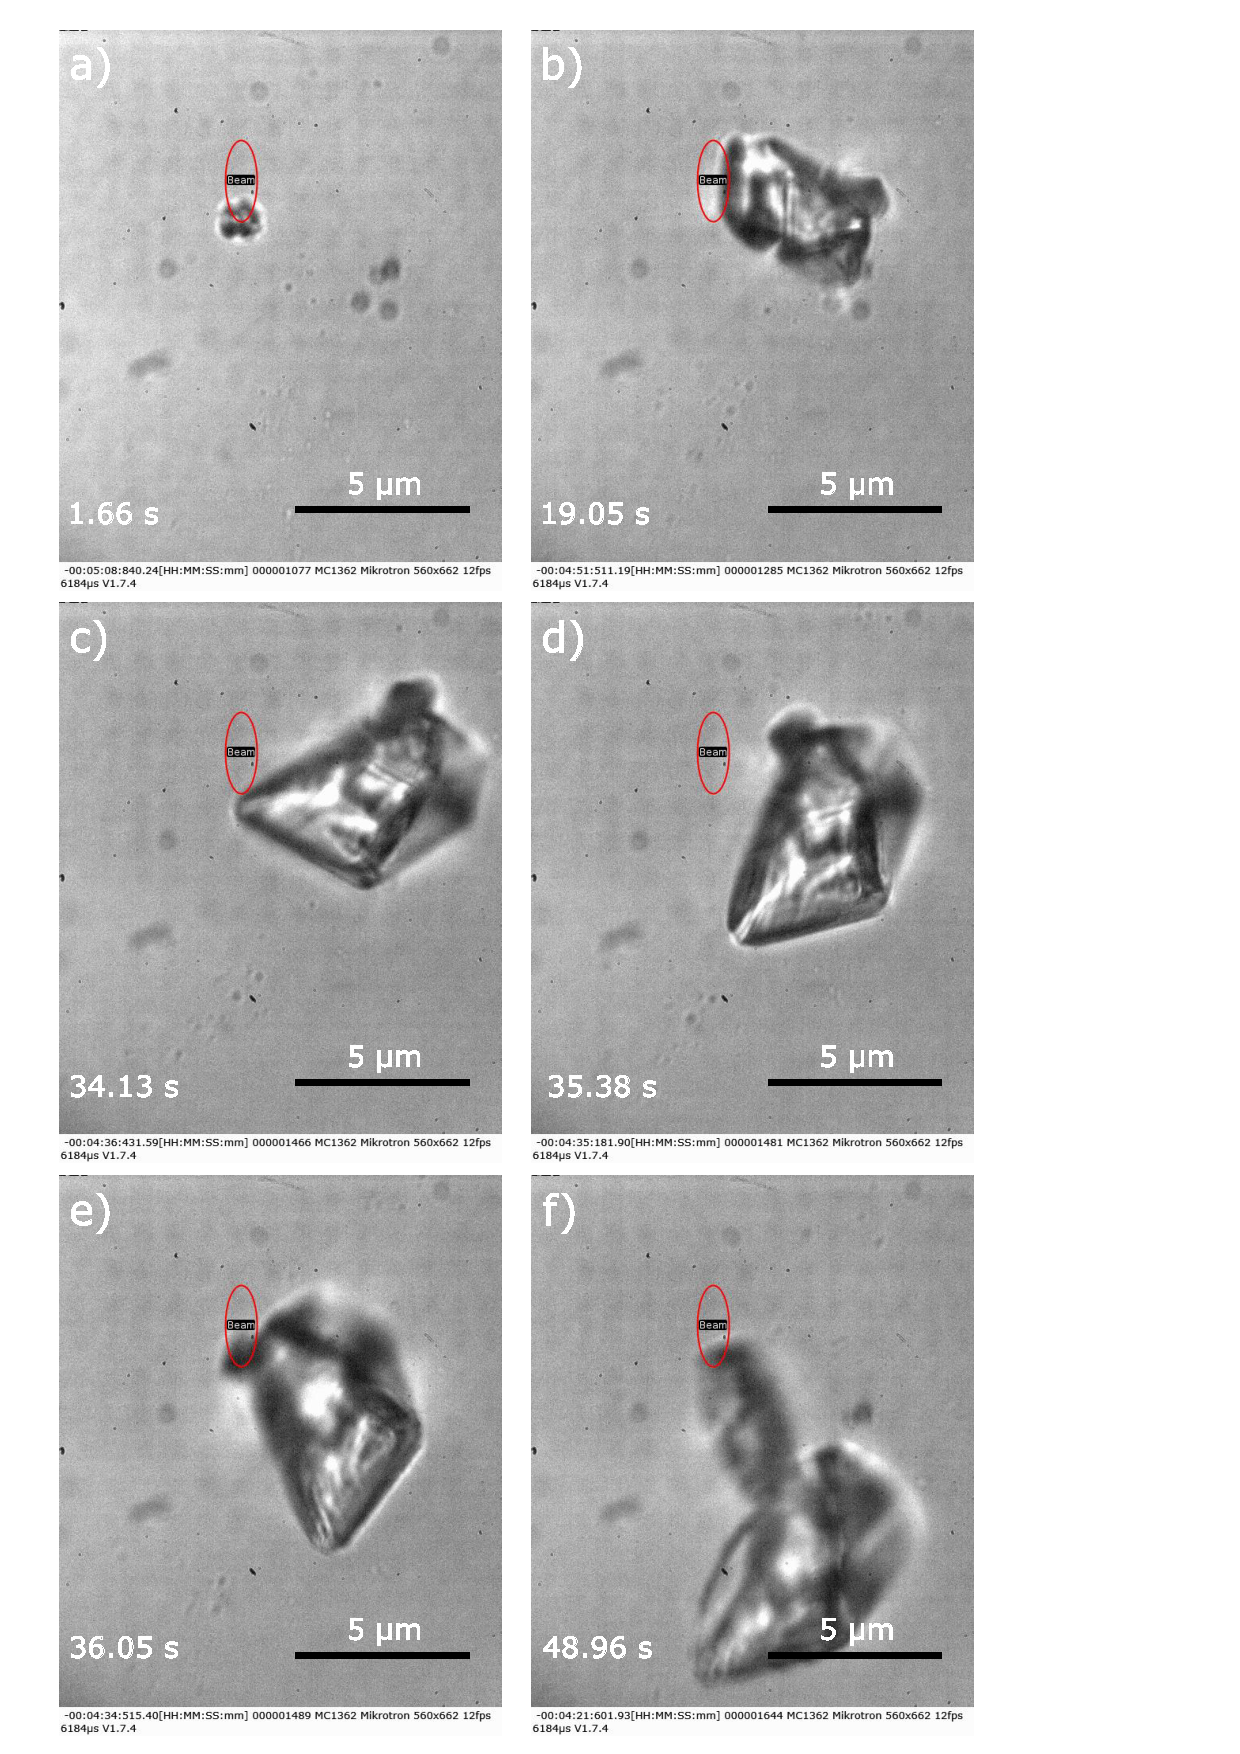
\includegraphics[width=0.9\linewidth]{frames_eliptical_beam.pdf}
	\caption{Laser induced nucleation at the edge of a droplet of 
		supersaturated glycine solution. (b) shows the first instance 
		of a crystal nucleus, growing quickly through (c)-(e) until 
		after $6.665\ s$ the crystal begins to escape the trap.}
	\label{fig:eliptical_beam_1}
\end{figure}

In this instance $20\ \mu L$ of glycine and water ($S=1.03$) was added to $10\ \mu L$ 
of a dilute water-silica mixture making the solution undersaturated ($S\approx0.7$). 
Nucleation in undersaturated conditions has been reported previously in $D_2O$ 
\cite{Rungsimanon2010} and $H_2O$ \cite{Flannigan2023}. Though notably in both cases the
crystal morphology is not influenced by the location of the laser focus, it has been
shown that polarisation can influence the polymorphic control for simple salts 
\cite{Garetz1996, Garetz2002} but no research has been done into the influence of a 
moving beam front on the growth of a newly formed nucleus.  


\section{Influence of a moving beam front on seed crystals}
To see if the above phenomena had any direct influence on a  